%  LaTeX support: latex@mdpi.com
%  MDPI MAKE submission — main_paper_MAKE44.tex
%  Version 44: revisions in response to review43.md
%    - [R1] Appendix A.1: D_j(R_j) redefined as the residual variance
%      contribution (not "distortion reduction"); R_j in nats; L_j stated
%      as maximized up to additive constants; lambda_j / tau^2 defined
%    - [R11] aggregated-posterior mismatch on active coordinates stated as
%      "assumed negligible" at the specific linear-Gaussian optimum
%    - [R12] "underestimating truncation" reworded: surrogate tends to
%      predict weaker truncation / may overestimate active dimensions
%    - [R2] d*(beta) > 512 restated as observation + surrogate-consistent
%      interpretation (d*_eff(beta) > 512); Sec. 1.2 contribution likewise
%    - [R3] "clear induced saturation" -> reduction in activation ratio /
%      stronger truncation within tested range; no stable-plateau claim
%    - [R4] Figure fig:en regenerated (EN_conv_vae_extended_m_v44) with
%      "Step-1 ref. \hat d_ID = 10" label; caption notes the reference-AE
%      origin of the value (Figs. 2/3 already render \hat d_ID)
%    - [R5] "safe-side operation" -> conservative operating strategy
%    - [R6][R7] abstract: seed design made explicit (3-5 synthetic /
%      3 real); "three steps ... reproducible decision rule" limited to
%      the pre-specified Step-3 rule + complementary MSE diagnostics
%    - [R8] Sec. 5.3.3: AE window [10,24] derivation made reproducible
%      (round(TwoNN)=10; ceil(2*MLE)=24), flagged as MNIST-specific
%    - [R9] Sec. 4.1: \hat d_ID as practical reference point, not a formal
%      lower bound for real data
%    - [R13][R14] Torus: "self-intersecting (an immersion)" weakened to
%      consistency statement; "deterministic" -> identical across the five
%      tested seeds
%    - [R15] Table tab:applicability: "Fully applicable" -> ground-truth
%      validated with an adaptive margin diagnostic
%    - [R16] Table tab:failure: "Likely cause" -> "Diagnostic
%      interpretation"; lower-V2 row reworded as consistency statement
%    - [R17] m_ref ~ 2 \hat d_ID on natural images labeled a provisional
%      consistency region, not a validated selection rule
%    - [R18] Allegra et al.: "model exactly" -> "provide a related
%      treatment of"
%    - [R19] Table tab:notation: d_emb entry now relates to ideal manifold
%      dimension d (not d_ID)
%    - [R20] Fig. 2 caption: single-seed sweep for visualization; principal
%      verification decisions from 3-seed Table tab:mnist_s3 / Fig. 3
%    - [R21] "organized into three contributions" fixed
%    - [R22] Sec. 4 title -> "Theoretical Motivation and Interpretive
%      Surrogates"
%    - [R23] DANCo claim conditioned; [R24] "the manifold dimension" in the
%      Introduction replaced by an estimate of local intrinsic
%      dimensionality
%    - [R25] Sec. 5.1: +/- values are inter-seed standard deviations
%    - [R26] "identical"/"unanimous" -> explicit per-seed statements
%  ---- Version 43 changes below ----
%  Version 43: revisions in response to
%  MAKE投稿論文_修正指摘と改善案.md (pre-submission review)
%    - [T1] title changed from "Choosing ... from the Intrinsic Dimension"
%      to "Intrinsic-Dimension-Guided Bottleneck Selection ... with
%      Active-Unit Diagnostics" (protocol/diagnostics framing)
%    - [T2] abstract rewritten: conditional diagnostic protocol; VAE rule
%      m >= 2*dID stated as generous-candidate + post-training check, not a
%      guarantee; "grid-best" -> "best observed"; AU explicitly not a
%      general estimator of intrinsic/embedding dimension
%    - [T4] Prop. 1 restricted to idealized zero-error continuous
%      reconstruction; d_emb >= d_ID framed as geometric motivation, not an
%      empirically verifiable inequality involving \hat d_ID; Prop. 2
%      explicitly not a coordinate-wise activation theorem for nonlinear
%      VAEs; ELBO-surgery exactness limited to the specific global optimum;
%      Prop. 3 demoted to a heuristic conditional-stability rationale
%      (no Proposition environment; all cross-references updated)
%    - [T5] AUsat notation-table entry reworded; AU coordinate dependence
%      (non-invariance under latent rotations/reparameterizations) added
%    - [T6] Step-1 reference AE vs Step-3 candidate VAE separation made
%      explicit; single-seed m_ref sweep vs 3-seed verification clarified;
%      subsampling-CI scope limited; "stable" claims conditioned on the
%      tested datasets/architectures/estimators
%    - [T7] V1/V2 restated as operational screening criteria; explicit
%      list of what a pass does NOT imply
%    - [T8] training-run accounting table added (Table tab:cost);
%      VAE 0.9-point gap quantified, no equivalence claim; AE single-seed
%      probe results flagged as descriptive
%    - [T9] fixed-beta surrogate vs cyclical KL annealing distinguished
%      (beta_max = schedule parameter); annealing schedule specified;
%      natural-image mechanisms framed as untested hypotheses with an
%      operational definition of manifold entanglement; SVHN raw-input
%      TwoNN not treated as ground truth; tau_eff^2 flagged post hoc
%    - [T10] fixed-order subset rationale and caveat added
%    - [T11] related work extended: ID-estimator limitations
%      (Camastra & Staiano 2016; Allegra et al. 2020) and AU definition
%      limits
%    - [T12] Table tab:ea simplified (notes moved to caption); Figure
%      fig:e4_dualaxis split into 4 panels (E4_mnist_dualaxis_v43);
%      Figure fig:e4_multiseed labels reworded (E4_300ep_multiseed_v43);
%      Figure fig:ep caption no longer suggests isometry is irrelevant
%    - [T13] Sec. 1.2 contributions reorganized (methodological /
%      diagnostic / empirical / theoretical motivation); Sec. 1.4 trimmed
%  ---- Version 42 changes (in response to Peer_Review_Report41.md) below ----
%    - [Major 2] Fashion-MNIST Step 3 upgraded to a 3-seed verification
%      (Exp-Fashion-MS, 300 ep)
%    - [Major 2] Exp-ConvV-HiBeta upgraded to a 3-seed verification
%      (Exp-ConvV-HiBeta-MS)
%    - [Major 1] hypotheses on why latent-geometry distortion is so
%      pronounced on natural images (manifold entanglement, need for
%      hierarchical latents) added to Secs. 5.6.2 and 6.4
%    - [Major 3] discussion of the aggregated-posterior mismatch
%      KL(q(z)||p(z)) during nonlinear optimization added to Remark 2 and
%      Appendix A.1 (ELBO surgery reference added)
%    - [Minor 1] abstract: specific numbers trimmed, emphasis shifted to
%      the closed-loop protocol
%    - [Minor 2] Figures 2 (E4_300ep_multiseed) and 5 (Exp_ConvV_HiBeta)
%      regenerated with B/W-print-safe line styles and larger fonts
%    - [Minor 3] Step 2: the multiplier 2 re-emphasized as a buffer for the
%      unknown d_emb
%  ---- Version 41 changes (in response to Review_codex40.txt) below ----
%    - DANCo wording in Sec. 2 fixed: not a primary estimator, used as an
%      auxiliary robustness cross-check on MNIST latents (Minor 1)
%    - full audit of references (all cited, citation-order numbering) and
%      of figure/table in-text mentions
%  ---- Version 40 changes (in response to Review_codex39.txt) below ----
%    - Sec. 4 real-data-validation question rephrased: "does the full
%      protocol work on MNIST, what evidence is available for
%      Fashion-MNIST" (Minor 1)
%    - repository URL/DOI (Minor 2) and MDPI production placeholders
%      (presentation 1) left for the submission/editorial stage
%  ---- Version 39 changes (in response to Review_codex38.txt) below ----
%    - contradictory Fashion-MNIST sentence in Sec. 4.3.6 rewritten:
%      Step 1 is multi-seed, VAE-side AU verification is a single-seed
%      preliminary observation (Minor 1)
%    - Sec. 4.1 multi-seed sentence refined to "used for the principal
%      verdicts"; in-text exploratory single-seed summaries acknowledged
%      (Minor 2)
%    - Sec. 4.3.3 parenthetical added: AE window = TwoNN--MLE envelope,
%      VAE m_ver = primary TwoNN rule (Minor 3)
%    - Sec. 1.2 contribution claim made exact: multi-seed AU verification
%      on MNIST; Step-1 stability via subsampling CIs, estimator
%      cross-checks, and the 3-seed reference-model comparison (Minor 4)
%    - V2 threshold-invariance note: displayed range rounded conservatively
%      (mean lower edge 2.24) (presentation 2)
%    - natural-image table caption: Pope et al. agreement limited to
%      CIFAR-10 (presentation 3)
%    - abstract boundary-case detail lightly trimmed (presentation 4)
%    - MDPI production placeholders (dates, article no., DOI) left
%      for the editorial stage (presentation 1); author ORCID iDs filled in
%  Compiled with official mdpi.cls
%  Compile: pdflatex main_paper_MAKE42.tex  (x3 for cross-references)

%=================================================================
\documentclass[make,article,submit,pdftex,moreauthors]{Definitions/mdpi}

%=================================================================
% MDPI internal commands — do not modify
\firstpage{1}
\makeatletter
\setcounter{page}{\@firstpage}
\makeatother
\pubvolume{8}
\issuenum{1}
\articlenumber{0}
\pubyear{2026}
\copyrightyear{2026}
%\externaleditor{Firstname Lastname}
\datereceived{ }
\daterevised{ }
\dateaccepted{ }
\datepublished{ }

%=================================================================
% Notation shorthands (kept in sync with main_paper_NN35.tex)
\newcommand{\dID}{d_{\mathrm{ID}}}
\newcommand{\hatdID}{\hat{d}_{\mathrm{ID}}}
\newcommand{\dz}{m}
\newcommand{\dtrue}{d_{\mathrm{true}}}
\newcommand{\Jg}{J_g}
\newcommand{\R}{\mathbb{R}}
\newcommand{\kap}{\kappa}
\newcommand{\AUsat}{\mathrm{AU}_{\mathrm{sat}}}
\newcommand{\demb}{d_{\mathrm{emb}}}
\newcommand{\mknee}{m^{\mathrm{knee}}}
\newcommand{\dstar}{d^{*}(\beta)}

%=================================================================
\Title{Intrinsic-Dimension-Guided Bottleneck Selection for Autoencoders
and Variational Autoencoders with Active-Unit Diagnostics}

% ORCID IDs
\newcommand{\orcidauthorA}{0009-0001-1209-0918} % Chika Obata
\newcommand{\orcidauthorB}{0000-0002-4070-4585} % Mizuki Dai
\newcommand{\orcidauthorC}{0000-0002-0431-5769} % Kenya Jin'no

\Author{Chika Obata $^{1}$\orcidA{},
        Mizuki Dai $^{1}$\orcidB{}, and
        Kenya Jin'no $^{1,}$*\orcidC{}}

\AuthorNames{Chika Obata, Mizuki Dai, and Kenya Jin'no}

\address{%
$^{1}$ \quad Department of Intelligent Systems,
  Faculty of Information Engineering,
  Tokyo City University,
  1-28-1 Tamazutsumi, Setagaya-ku, Tokyo 158-8557, Japan;
  g2332016@tcu.ac.jp (C.O.); g2591402@tcu.ac.jp (M.D.)}

\corres{Correspondence: kjinno@tcu.ac.jp; Tel.: +81-3-5707-0104 (K.J.)}

%=================================================================
\abstract{%
The bottleneck dimension $m$ is a fundamental design choice in autoencoders
(AEs) and variational autoencoders (VAEs), yet in practice it is usually
selected by convention or trial and error.
We propose a \textbf{conditional, diagnostic protocol} that uses an
estimate $\hatdID$ of the intrinsic dimension of the input data as a
data-dependent \textbf{search-window reference} for selecting $m$.
For AEs, the protocol recommends searching within a finite window centered
on $\hatdID$, typically $m \in [\hatdID, 2\hatdID]$; for VAEs, it
recommends selecting a sufficiently generous candidate dimension
$m \geq 2\hatdID$ and verifying post training whether the surplus
coordinates became inactive, using active units (AU) and reconstruction
error.
The geometric motivation is a topological lower bound for zero-error
continuous reconstruction of an idealized manifold; the VAE-side
interpretation is supported by a linear-Gaussian rate--distortion surrogate
with activation condition $\lambda_j > \beta\tau^2$.
On synthetic manifolds with known ground truth (three to five seeds) and on
fully connected VAEs trained on MNIST and Fashion-MNIST (three seeds each),
the protocol produced reproducible diagnostics, using a pre-specified Step-3
screening rule for VAEs together with complementary reconstruction-error
diagnostics (MNIST passes; on Fashion-MNIST the rule
diagnostically detects an over-pruning boundary case), and on the specific
MNIST grid used here the ID-guided window reduces the training runs of a
full grid search by roughly 60--80\% while containing the best observed
linear-probe accuracy.
The method is conditional rather than universal: under the datasets,
architectures, and estimators tested, intrinsic-dimension estimates were
numerically stable only through reference representations with
$m \gg \hatdID$ and inflate on natural images, and for Conv-VAEs the AU
truncation fails at standard $\beta$, with $\beta$-strengthening restoring
truncation (3 seeds) but not order consistency.
These results support using $\hatdID$ as a search-window reference and AU
as a \textbf{model- and training-dependent diagnostic}---not as general
estimators of intrinsic or embedding dimension.}

\keyword{variational autoencoder; bottleneck dimension; intrinsic dimension;
manifold hypothesis; active units; TwoNN; diagnostic protocol;
model selection; representation learning; knowledge extraction}

%=================================================================
\begin{document}

\section{Introduction}\label{sec:intro}

\subsection{Background: How Should the Bottleneck Dimension Be Chosen?}\label{sec:intro_bg}

Autoencoders (AEs) and variational autoencoders
(VAEs)~\cite{kingma2014vae} are core unsupervised models that learn
low-dimensional latent representations from high-dimensional
data~\cite{bengio2013representation}.
Their most fundamental design parameter is the bottleneck dimension $m$:
if $m$ is too small, information is lost; if it is too large, redundant
dimensions arise and, in VAEs, complicate the interpretation of posterior
collapse~\cite{lucas2019elbo}.
Nevertheless, in practice $m$ is usually set to ``a round number such as 32
or 64'' or tuned by trial and error, and a selection principle grounded in
the data itself has not been established.

On the other hand, according to the manifold
hypothesis~\cite{fefferman2016manifold}, natural data concentrate near a
low-dimensional manifold inside the high-dimensional input space $\R^N$,
and the local number of degrees of freedom is characterized by the intrinsic
dimension $\dID \ll N$.
Indeed, estimators such as TwoNN~\cite{facco2017twonn} report that the
intrinsic dimension of natural images is far smaller than the pixel
dimension~\cite{pope2021intrinsic}.
From this viewpoint, \textbf{the appropriate scale of the bottleneck
dimension $m$ should be informed not by model-side convention but by a
data-side geometric quantity---namely, an estimate of the local intrinsic
dimensionality}.
The question addressed in this paper is:
\begin{quote}
\textit{Can the bottleneck dimension $m$ of an AE/VAE be chosen in a
principled way from an estimate of the intrinsic (manifold) dimension of the
input data?
And is there a means of verifying, after training, that the choice was
appropriate?}
\end{quote}

\subsection{Central Idea and Contributions}\label{sec:intro_aim}

The central claim of this paper can be stated in one sentence:
\begin{quote}
\textbf{An estimate $\hatdID$ of the intrinsic dimension of the input data
provides a search-window reference for the bottleneck dimension $m$---%
``AE: $m \in [\hatdID,\, 2\hatdID]$; VAE: a generous candidate
$m \geq 2\hatdID$''---and the active units (AU) of a VAE---the number of
coordinates actually used under KL regularization---serve, under a suitable
$\beta$ and architecture, as a post-training diagnostic of whether the
surplus dimensions were actually truncated.}
\end{quote}
This is not a claim of a general solution to choosing $m$, nor a
single-number selection algorithm; it is the proposal of a
\textbf{conditional diagnostic protocol}
(applicability conditions are summarized in
Table~\ref{tab:applicability}).
In particular, $\hatdID$ provides the center or lower side of a candidate
range rather than a unique correct answer, the VAE-side rule
$m \geq 2\hatdID$ is neither a sufficient condition nor an optimality
principle (in practice the candidate is picked from a finite pre-specified
grid), and AU is not an estimator of intrinsic or embedding dimension but a
diagnostic that depends on $\beta$, the AU threshold, the architecture, and
the training conditions.
Within the linear-Gaussian surrogate of Section~\ref{sec:theory}, the
activation condition $\lambda_j > \beta\tau^2$
(Proposition~\ref{thm:linear_vae}) predicts that even if $m$ is set above
the required dimension, the KL regularization of the VAE truncates the
surplus dimensions (posterior collapse) and the AU count reports the
effective number of used dimensions---in other words,
\textbf{whereas for an AE the choice of $m$ itself fixes the representation
dimension, for a VAE the conservative operating strategy of using a generous
candidate dimension followed by AU-based verification can be expected to
apply} (whether this expectation actually holds is
itself checked by the Step-3 decision rule).

The contributions and theoretical motivation of this paper are organized as
follows:
\begin{enumerate}
  \item \textbf{Methodological contribution: an ID-guided
        bottleneck-dimension selection protocol}
        (Section~\ref{sec:protocol}): an estimate--set--verify workflow
        consisting of
        (S1) estimating $\hatdID$ (TwoNN/MLE; for real data through a
        reference AE with $m_{\mathrm{ref}} \gg \hatdID$),
        (S2) setting $m$ (AE: $m \in [\hatdID, 2\hatdID]$ plus a topological
        margin; VAE: a generous setting $m \geq 2\hatdID$), and
        (S3) post-training verification by AU and reconstruction error,
        together with a \textbf{reproducible pass/fail decision rule}
        (Equations~\eqref{eq:rule_v1}--\eqref{eq:rule_v2}) and reporting
        requirements.
  \item \textbf{Diagnostic contribution}: a failure-mode taxonomy
        (Table~\ref{tab:failure}) that combines AU and MSE to distinguish
        surplus-dimension truncation, over-regularization, Step-1
        underestimation, and topological obstructions, demonstrated on
        ground truth (Torus over-pruning caught by the MSE cross-check) and
        on real data (Fashion-MNIST lower-V2-bound violation).
  \item \textbf{Empirical contribution: multi-seed validation and
        quantified applicability boundaries} (Section~\ref{sec:exp}):
        the full protocol is validated on synthetic manifolds with known
        ground truth (3--5 seeds) and on fully connected VAEs on MNIST
        (3 seeds; $\hatdID \approx 10$--12 consistent with the AU slowdown
        region), with Step-1 stability supported by subsampling confidence
        intervals, cross-checks with estimators of different principles
        (DANCo, ESS), and a 3-seed reference-model comparison
        (Section~\ref{sec:exp_real_geom}); a linear probe shows that on the
        specific MNIST grid tested here the ID-guided range reduces search
        cost while containing the best observed downstream accuracy
        (Section~\ref{sec:exp_downstream}).
        The applicability limits are quantified in the same experiments:
        (a) under the tested datasets, architectures, and estimators,
        $\hatdID$ was numerically stable only through reference
        representations with $m \gg \hatdID$, while isometry improvements
        were secondary (Section~\ref{sec:exp_real_geom});
        (b) on natural images the TwoNN estimate agrees with reported
        values~\cite{pope2021intrinsic} up to $m \approx 2\hatdID$ but
        inflates beyond;
        (c) for Conv-VAEs at $\beta_{\max} = 4$ no substantial truncation
        is observed within $m \leq 512$---consistent, under the surrogate
        interpretation, with an effective truncation threshold beyond the
        tested range---so AU verification requires a strengthened
        $\beta$ (the $\beta$-strengthened recovery achieves V1 only, not
        V2; 3 seeds), and Step 3 on natural images remains unresolved---the
        contributions are claimed inclusive of these limitations.
  \item \textbf{Theoretical motivation} (Section~\ref{sec:theory}):
        an idealized topological lower bound for zero-error continuous
        reconstruction (Proposition~\ref{thm:lower_bound}) and the
        surrogate activation condition $\lambda_j > \beta\tau^2$ under a
        linear-Gaussian rate--distortion approximation
        (Proposition~\ref{thm:linear_vae}).
        Both are motivations rather than guarantees for trained nonlinear
        networks: the lower bound assumes zero reconstruction error and
        continuity, and the activation condition is exact only for the
        linear-Gaussian surrogate (its scope is stated in the claim
        bodies).
\end{enumerate}

\textbf{Relation to prior work}:
studies that ``measure'' the intrinsic dimension of deep
representations~\cite{ansuini2019intrinsic,pope2021intrinsic,valeriani2023geometry}
stop at analyzing trained networks, whereas this work uses
intrinsic-dimension estimation for the \textbf{design of the bottleneck
dimension} and formalizes a closed-loop verification of that design through
AU.
Whereas the linear analysis of posterior collapse~\cite{lucas2019elbo}
remains qualitative, we organize it into the closed-form threshold
$\lambda_j > \beta\tau^2$ (the novelty lies in the integrated organization;
Section~\ref{sec:theory}) and operate it as the rationale of the selection
protocol.

\subsection{Two Faces of the ``Manifold Dimension'': $\dID$ and $\demb$}\label{sec:intro_dim}

As the ``manifold dimension of the input data'' we distinguish two
quantities:
the \textbf{local intrinsic dimension} $\dID$ (the local degrees of freedom
of the manifold; the target of TwoNN/MLE) and the
\textbf{topological minimum embedding dimension} $\demb$ (the minimum
dimension for embedding into Euclidean space without self-intersection).
For the Swiss Roll $\demb = \dID = 2$, but for the Torus
$\demb = 3 > \dID = 2$.
What the bottleneck requires is $\demb$
(Proposition~\ref{thm:lower_bound}); since only $\dID$ can be estimated for
real data, this gap (topological obstruction) is one reason for the margin
``set $m$ above $\hatdID$'' (Section~\ref{sec:protocol_s2}).
One caution applies throughout: for an ideal $d$-dimensional smooth
manifold the minimum Euclidean embedding dimension satisfies
$\demb \geq d$, but in real datasets $\hatdID$ is an estimator of
\textbf{local intrinsic dimensionality}, not a direct estimator of
$\demb$.
The relation between intrinsic and embedding dimensions should therefore be
read as a \textbf{geometric motivation for adding a margin}, not as an
empirically verifiable inequality involving $\hatdID$.

\subsection{Limitations of This Paper (Summary)}\label{sec:intro_limits}

Our validation covers synthetic manifolds with known ground truth
($\dtrue \leq 3$), MNIST and Fashion-MNIST (fully connected AE/VAE,
3 seeds), and---as quantification of the applicability boundary---Conv-VAEs
and natural images (CIFAR-10, SVHN).
The state of validation is asymmetric: \textbf{fully connected
architectures receive complete multi-seed validation}, whereas
\textbf{convolutional architectures and natural images are at the stage of
probing the applicability boundary} (a 3-seed $\beta$-strengthening
experiment and single-seed exploratory observations).
Two further caveats recur throughout: a numerically stable $\hatdID$ is not
necessarily unbiased (stability vs.\ validity;
Section~\ref{sec:disc_twonn}), so $\hatdID$ is operated as a
\textbf{reference value}, not as the true value; and automatic change-point
(knee) detection on the AU curve is strongly grid- and seed-dependent, so
it is not a named protocol output (exploratory analysis in
Appendix~\ref{app:knee}).
Full application to large-scale natural images remains future work; a
detailed discussion of limitations is given in
Section~\ref{sec:disc_limitation}.

The remainder of the paper covers related work (Section~\ref{sec:related}),
the protocol (Section~\ref{sec:protocol}), its theoretical motivation
(Section~\ref{sec:theory}), experiments (Section~\ref{sec:exp}), discussion
(Section~\ref{sec:discussion}), and conclusions
(Section~\ref{sec:conclusion}).
Proofs, sensitivity analyses, and exploratory experiments are collected in
the appendices.

%% ===================================================================
\section{Related Work}\label{sec:related}

\textbf{Representation learning and autoencoders}:
Bengio et al.~\cite{bengio2013representation} organized the framework in
which AEs learn the low-dimensional structure of high-dimensional data based
on the manifold hypothesis~\cite{fefferman2016manifold}.
The $\beta$-VAE~\cite{higgins2017betavae} controls the degree of compression
of the representation through the KL weight $\beta$, which directly affects
AU.
DAE~\cite{alain2014dae} and CAE~\cite{rifai2011cae} are regularized variants
that promote learning of manifold structure; in this paper they serve as
candidate reference representations for intrinsic-dimension estimation
(Section~\ref{sec:exp_real_geom}).

\textbf{Intrinsic-dimension analysis of deep representations}:
Pope et al.~\cite{pope2021intrinsic} showed that the intrinsic dimension of
natural images is far lower than the pixel dimension (CIFAR-10:
$\dID \approx 26$), and Ansuini et al.~\cite{ansuini2019intrinsic}
quantified how the ID changes across layers of deep networks.
Valeriani et al.~\cite{valeriani2023geometry} analyzed the hidden-representation
geometry of large transformers, and Birdal et
al.~\cite{birdal2021intrinsic} related ID to generalization.
These are studies that ``measure'' trained models; our work is complementary
in that it uses the measurements for the \textbf{design and verification of
the bottleneck dimension}.
As ID estimators we adopt TwoNN~\cite{facco2017twonn} and
MLE~\cite{levina2005mle}; DANCo~\cite{ceruti2014danco} can provide a useful
complementary estimator but is computationally more expensive, so we do not
use it as a primary estimator and
instead apply it as an auxiliary robustness cross-check on selected MNIST
latents (Section~\ref{sec:exp_mnist_ci}).

\textbf{Limitations of intrinsic-dimension estimators}:
nearest-neighbor ID estimators are known to suffer from finite-sample bias,
sensitivity to non-uniform sampling, noise, and curvature, and from
distance concentration when the ambient dimension is large relative to the
sample size (see the survey by Camastra and
Staiano~\cite{camastra2016intrinsic}).
Real data may moreover be better described as a union of submanifolds with
heterogeneous local intrinsic dimension, which conflicts with the
single-manifold assumption underlying global
estimators~\cite{allegra2020data}, and estimates computed on deep
representations depend on the representation
itself~\cite{ansuini2019intrinsic,pope2021intrinsic}.
Our experiments encounter all of these effects (sample-size-dependent bias
in Section~\ref{sec:exp_mnist_ci}; representation dependence in
Sections~\ref{sec:exp_real_geom} and \ref{sec:exp_boundary}), which is why
the protocol treats $\hatdID$ as a conditional reference value with
mandatory convergence and cross-estimator checks rather than as a trusted
point estimate.

\textbf{Active units and posterior collapse}:
AU~\cite{higgins2017betavae,lucas2019elbo} is the number of latent
dimensions whose posterior-mean variance exceeds a threshold $\delta$, and
measures the number of coordinates actually used under KL regularization.
Lucas et al.~\cite{lucas2019elbo} analyzed the mechanism of posterior
collapse in linear VAEs.
This work incorporates that mechanism into the selection protocol as a
``safety device that can truncate an over-generous $m$'' (whether truncation
actually occurred is diagnosed in Step 3), with the water-filling activation
condition as its theoretical rationale
(Proposition~\ref{thm:linear_vae}; the PPCA of Tipping \&
Bishop~\cite{tippingbishop1999ppca} is the special case $\beta = 1$).

\textbf{Automatic determination of the number of latent dimensions}:
within linear and probabilistic models, Bayesian PCA with an ARD (automatic
relevance determination) prior~\cite{bishop1999bayesian} determines the
number of principal components, and Bayesian nonparametric latent variable
models such as those based on the Indian Buffet
Process~\cite{ghahramani2005infinite} determine the number of latent
features, during learning.
The KL truncation of the $\beta$-VAE performs a similar ``automatic pruning
of surplus dimensions'' in the nonlinear setting, but the pruning result
depends on $\beta$ and the architecture (Section~\ref{sec:exp_boundary}).
Rather than relying on model-side automatic determination, our protocol
derives a search window from the data-geometry side ($\hatdID$) and
verifies it against the pruning result (AU); the two approaches are
complementary.

\textbf{Geometric autoencoders}:
Nazari et al.~\cite{nazari2023geometric} and Kato et
al.~\cite{kato2020rdae} proposed regularizers that preserve the geometry
(isometry) of the latent space.
We compare the effect of isometry on the stability of ID estimation against
the ``bottleneck margin $m / \hatdID$'' and show that the latter is dominant
(Section~\ref{sec:exp_real_geom}).

%% ===================================================================
\section{ID-Guided Protocol for Selecting the Bottleneck Dimension}\label{sec:protocol}

\subsection{Problem Setting and Main Symbols}\label{sec:protocol_setup}

We define an AE/VAE with input dimension $N$, bottleneck dimension $m$,
encoder $f: \R^N \to \R^m$, and decoder $g: \R^m \to \R^N$.
In a VAE the encoder outputs a posterior
$q_\phi(z|x) = \mathcal{N}(\mu(x), \sigma^2(x))$, and the KL regularization
(strength $\beta$) acts as an information bottleneck.

We define the \textbf{active units (AU)} as
\begin{equation}
  \mathrm{AU}(m) = \sum_{k=1}^{m} \mathbf{1}\bigl[\mathrm{Var}_x[\mu_k(x)] > \delta\bigr],
  \quad \delta = 10^{-2},
  \label{eq:au_def}
\end{equation}
where $\mu_k(x)$ is the $k$-th component of the posterior mean; the
threshold $\delta$ follows Lucas et al.~\cite{lucas2019elbo}, and we have
confirmed that AU values are essentially unchanged for
$\delta \in [10^{-3}, 10^{-1}]$ (Appendix~\ref{app:sens}).
AU is computed on test data (the train/test distinction is stated in each
experiment section).
Three definitional remarks on AU apply throughout.
First, AU is based on the data variance of the \textbf{posterior mean};
it is not identical to a per-coordinate decomposition of the posterior
variance or of the KL contribution.
Second, the threshold $\delta$ is compared against latent-coordinate
variances and can in principle depend on the latent scale (in our settings
the standard-normal prior anchors the scale, and the
$\delta$-insensitivity above holds).
Third, \textbf{AU is coordinate-dependent}: it is not invariant under
arbitrary rotations or reparameterizations of the latent space, so its
interpretation depends on the chosen prior, parameterization, training
objective, and architecture.

\begin{table}[H]
\caption{Main symbols. Each quantity is distinguished so that the protocol's
claims are stated without conflating targets and estimators.}
\label{tab:notation}
\small
\begin{tabular}{lp{5.6cm}p{4.9cm}}
\toprule
\textbf{Symbol} & \textbf{Meaning} & \textbf{Role in the protocol} \\
\midrule
$m$ & Bottleneck dimension & Design parameter to be chosen \\
$\dID$ & Intrinsic dimension of the data manifold & Target quantity (unknown for real data) \\
$\demb$ & Minimum Euclidean embedding dimension of the specified manifold; for an ideal $d$-dimensional manifold, $\demb \geq d$ & Lower bound for $m$ (Prop.~\ref{thm:lower_bound}) \\
$\hatdID$ & TwoNN/MLE estimate of $\dID$ & \textbf{Reference value} for Step 1 (may be biased) \\
$\mathrm{AU}(m)$ & Number of KL-active coordinates, Equation~\eqref{eq:au_def} & Verification signal for Step 3 \\
$\AUsat$ & Saturated (plateau) AU value & Saturated number of empirically active coordinates under the specified $\beta$, $\delta$, and architecture (VAE) \\
$\dstar$ & Water-filling threshold count (Prop.~\ref{thm:linear_vae}) & Idealized prediction of $\AUsat$ \\
$\kap$ & Decoder Jacobian condition number & Isometry (distortion) indicator \\
\bottomrule
\end{tabular}
\end{table}

Two distinctions deserve emphasis here.
First, $\hatdID$ is a \textbf{reference value, not the true value}: even
when TwoNN/MLE is numerically stable (low variance), it may carry a
systematic bias due to geometric distortion of the reference representation
(stability vs.\ validity; Section~\ref{sec:disc_twonn}).
Second, AU is \textbf{not an estimator of the intrinsic dimension}: AU is an
observable---``the number of coordinates the KL regularization allowed to be
used''---and depends on $\beta$, $\delta$, and the architecture.
The protocol is designed to avoid over-reliance on any single indicator by
cross-checking these two quantities of different natures.

\subsection{The Protocol}\label{sec:protocol_main}

Figure~\ref{fig:protocol} summarizes the three steps; the following
subsections specify each step.

\begin{figure}[H]
\centering
\renewcommand{\arraystretch}{1.4}
\begin{tabular}{c}
  \fbox{\textbf{Input data} $\boldsymbol{X} \in \R^N$ (under the manifold hypothesis)} \\[3pt]
  $\Big\downarrow$ \\[1pt]
  \fbox{\parbox{0.78\linewidth}{\centering
    \textbf{Step 1: Estimate the intrinsic dimension} \\[1pt]
    Low-dimensional data: apply TwoNN/MLE directly in input space \\
    Real data: TwoNN/MLE on the latents of a reference AE
    ($m_{\mathrm{ref}} \gg \hatdID$) \\
    Check convergence over several $m_{\mathrm{ref}}$; report TwoNN and MLE
    $\Rightarrow$ reference value $\hatdID$
  }} \\[3pt]
  $\Big\downarrow$ \\[1pt]
  \fbox{\parbox{0.78\linewidth}{\centering
    \textbf{Step 2: Set the bottleneck dimension} \\[1pt]
    AE: search window $m \in [\hatdID,\, 2\hatdID]$ (includes topological margin) \\
    VAE: set generously, $m \geq 2\hatdID$ (KL truncation of surplus
    dimensions expected)
  }} \\[3pt]
  $\Big\downarrow$ \\[1pt]
  \fbox{\parbox{0.78\linewidth}{\centering
    \textbf{Step 3: Post-training verification} \\[1pt]
    VAE: decision rule V1 (AU$/m \leq 0.9$) and
    V2 ($\hatdID \leq$ AU $\leq 3\hatdID$), multi-seed \\
    AE: does the rapid MSE improvement stop around
    $m \approx \hatdID$--$2\hatdID$? (visual) \\
    On failure: diagnose with the failure-mode
    Table~\ref{tab:failure}
  }}
\end{tabular}
\caption{ID-guided protocol for choosing the bottleneck dimension $m$.
The protocol closes the loop: the data-side estimate $\hatdID$ determines
the design, and the model-side observable AU verifies the design after
training.}
\label{fig:protocol}
\end{figure}

\subsubsection{Step 1: Estimating the Intrinsic Dimension}\label{sec:protocol_s1}

For synthetic or low-dimensional data, TwoNN/MLE can be applied directly in
input space.
For high-dimensional real data (e.g., $N = 784$ for MNIST), direct
estimation becomes unstable due to distance concentration, so we estimate
\textbf{through the latent representation of a generous reference AE
($m_{\mathrm{ref}} \gg \hatdID$; $m_{\mathrm{ref}} = 256$ in this paper)}.
Two requirements are mandatory:
(i) confirm convergence of the estimate over several $m_{\mathrm{ref}}$
(e.g., $\{64, 128, 256\}$);
(ii) report two estimators with different principles (TwoNN and MLE) and
confirm they agree in order of magnitude.
For setting the window and the verification point in Steps 2--3, the
\textbf{pre-registered primary estimator is the converged TwoNN value
rounded to the nearest integer}; MLE (and, where computed, DANCo/ESS)
serve as cross-checks (how a diverging cross-check is handled is specified
in Step 3).
The reference representation used in Step 1 must be trained
\textbf{independently of the candidate VAE models evaluated in Step 3};
latent-space estimates reported for candidate VAEs (e.g.,
Table~\ref{tab:mnist_s3}) are diagnostic cross-checks and are never used to
define $\hatdID$.
That the condition $m_{\mathrm{ref}} \gg \hatdID$ is the dominant condition
for stable estimation is consistent with the conditional-stability
rationale of Section~\ref{sec:theory_twonn} and supported by the
experiments (Section~\ref{sec:exp_real_geom}).
Conversely, $m_{\mathrm{ref}} \lesssim 3\hatdID$ causes systematic
underestimation, and on natural images inflation occurs for
$m_{\mathrm{ref}} \gg 2\hatdID$ (Section~\ref{sec:exp_boundary})---note that
the trust region of Step 1 is bounded in $m_{\mathrm{ref}}$.

\subsubsection{Step 2: Setting the Bottleneck Dimension}\label{sec:protocol_s2}

\textbf{For AEs}: for $m < \demb$, zero-error self-intersection-free
reconstruction is impossible in principle under the idealized
continuous-manifold assumption
(Proposition~\ref{thm:lower_bound}), and any excess
in $m$ remains as redundant dimensions (an AE has no automatic truncation).
We therefore take $m \in [\hatdID,\, 2\hatdID]$ as the \textbf{default
search window}, absorbing the possibility of a topological obstruction
($\demb > \dID$; Torus type) into the margin.
Here we re-emphasize the distinction of
Section~\ref{sec:intro_dim}: what the bottleneck actually requires is
$\demb$, but TwoNN/MLE can only estimate $\dID$, and $\demb$ is unknown for
real data.
\textbf{The multiplier 2 at the upper end of the window acts as a buffer
against this unknown gap $\demb - \dID$ (the topological
obstruction)}---$\hatdID$ must not be misread as an estimate of $\demb$.
Choose the upper side of the window if reconstruction accuracy matters, the
lower side if compression matters.
The factor 2 is not derived from first principles but is a default that
worked in our experiments; topology, noise, class mixtures, or
reconstruction-fidelity demands may require a larger margin (on the Torus,
activation stabilizes only at $m \geq 5 > 2\hatdID = 4$;
Section~\ref{sec:exp_syn})---the window is a starting point for the search,
not a guaranteed upper bound.

\textbf{For VAEs}: Proposition~\ref{thm:linear_vae} predicts, within the
surrogate model, that the KL regularization truncates surplus dimensions
even when $m$ exceeds the required dimension, so
\textbf{setting $m \geq 2\hatdID$ generously is the conservative operating
strategy}
(whether truncation actually occurred is checked by V1 in Step 3).
For the VAE, too, the role of the multiplier 2 is the same as for the AE: a
margin that keeps $m$ from falling below the unknown $\demb \geq \dID$ (as
long as truncation operates, any excess is reported post hoc by AU).
The truncation threshold, however, depends on $\beta$
($\dstar = |\{j : \lambda_j > \beta\tau^2\}|$): if $\beta$ is too small the
truncation fails and AU sticks at $m$ (detectable in Step 3).

\subsubsection{Step 3: Post-Training Verification}\label{sec:protocol_s3}

After training, the design is verified with two signals (both over multiple
seeds).

\textbf{VAE: AU verification (with a pass/fail decision rule)}.
The verification point $m_{\mathrm{ver}}$ is \textbf{pre-specified as the
smallest tested grid point $\geq 2\hatdID$---with $\hatdID$ the primary
TwoNN estimate of Step 1---before the AU curve is observed} (to avoid
post-hoc selection).
When a cross-check estimator (e.g., MLE) yields a $2\hatdID$ that falls
past the next grid point, verify there as well (on MNIST, MLE
$\approx 11.9$ points to $m = 32$ in addition to $m = 20$, and both pass;
Section~\ref{sec:exp_mnist}).
For a VAE trained at $m_{\mathrm{ver}}$, evaluate the following two
conditions on the multi-seed mean AU:
\begin{align}
  \text{V1 (truncation occurred)}:&\quad
  \mathrm{AU}(m_{\mathrm{ver}}) / m_{\mathrm{ver}} \leq 0.9,
  \label{eq:rule_v1}\\
  \text{V2 (order consistency)}:&\quad
  \hatdID \leq \mathrm{AU}(m_{\mathrm{ver}}) \leq 3\hatdID.
  \label{eq:rule_v2}
\end{align}
The verification \textbf{passes} when both hold (evidence of a compression
to the same order as the Step-1 intrinsic-dimension estimate);
failure of V1 suggests ``$\beta$ too small relative to the decoder
capacity,'' failure of the upper side of V2 suggests ``Step-1
underestimation or insufficient truncation,'' and failure of the lower side
suggests ``over-regularization ($\beta$ too large)''
(Table~\ref{tab:failure}).
V1 and V2 are \textbf{operational screening criteria introduced for this
study}: they are not hypothesis tests, confidence rules, or universally
calibrated acceptance criteria, and the threshold $0.9$ and factor $3$ are
working defaults.
In all settings of this paper, the verdicts on the multi-seed mean AU are
invariant for a V1 threshold in $(0.67, 0.94)$ and a V2 factor in
$(2.3, 6.8)$; recomputed per seed, all per-seed verdicts agree at the
default thresholds and are invariant for a V1 threshold in $(0.70, 0.93)$ and
a V2 factor in $(2.3, 6.6)$---the narrower per-seed V1 lower edge is set by
one MNIST seed with AU $= 14$ at $m_{\mathrm{ver}} = 20$.
The verdicts concerning the lower V2 bound (default coefficient 1) are
likewise invariant for a lower coefficient in $(0.70, 1.0]$, whose lower
edge is set by the Fashion-MNIST boundary case AU$/\hatdID = 0.70$
(Section~\ref{sec:exp_fashion}).
(Section~\ref{sec:exp}; the supplementary analysis script recomputes all
ranges; the displayed V2 ranges are rounded conservatively---the computed
mean-verdict lower edge is $2.23$.)
The width of the V2 band $[\hatdID, 3\hatdID]$ is a consequence of AU being
a $\beta$- and architecture-dependent observable rather than an ID
estimator (Section~\ref{sec:protocol_setup}); V2 checks order consistency
only, not that AU equals any dimension quantity---in particular, a pass
does not imply $\AUsat = \demb$ (see the Torus boundary behavior in
Section~\ref{sec:exp_syn}).
More generally, a V1/V2 pass indicates only that the observed AU is
compressed and of the same order as the Step-1 reference under the
specified conditions.
It does not establish that every surplus coordinate has fully collapsed,
does not establish equality between AU and the intrinsic or embedding
dimension, and does not guarantee reconstruction quality, generative
quality, or downstream utility; the rule is a diagnostic to be read
together with MSE (and, where relevant, ELBO, downstream metrics, and
visualization).
Simple manifolds show sharp saturation, while real data show a gradual
slowdown (Section~\ref{sec:exp_mnist}).

\textbf{MSE verification (qualitative diagnostic; AE and VAE)}.
Visually confirm that the rapid improvement of MSE$(m)$ slows down
around $m \approx \hatdID$--$2\hatdID$ (we do not propose an
algorithmic elbow detector; automatic change-point detection is
strongly grid- and seed-dependent and is confined to the exploratory
analysis of Appendix~\ref{app:knee}).
For VAEs the MSE verification must \textbf{always be read together with}
V1/V2: if AU passes but MSE keeps improving markedly beyond
$m_{\mathrm{ver}}$, suspect over-pruning due to a topological obstruction
($\demb > \dID$) and enlarge the margin (fifth row of
Table~\ref{tab:failure}; a concrete instance on the Torus is given in
Section~\ref{sec:exp_syn}).
The protocol is thus a \textbf{diagnostic workflow} that combines the
mechanical V1/V2 verdict with the required plots and statistics (see the
reporting requirements below); it is not a selection algorithm that outputs
a single number.

Failure modes for a mismatched verification are organized in
Table~\ref{tab:failure}; this is a diagnostic checklist for readers applying
the protocol to new data or architectures.

\begin{table}[H]
\caption{Failure modes in Step 3 and their diagnoses. Each row is backed by
the experiments in Section~\ref{sec:exp}.}
\label{tab:failure}
\small
\begin{tabular}{p{3.9cm}p{4.3cm}p{4.3cm}}
\toprule
\textbf{Symptom} & \textbf{Diagnostic interpretation} & \textbf{Remedy / follow-up} \\
\midrule
AU $= m$ for all tested $m$ (no truncation) & $\beta$ too small relative to decoder power ($\dstar \gg m$) & Increase $\beta$ or restrict decoder capacity; see Conv-VAE boundary (Section~\ref{sec:exp_boundary}) \\
AU saturates far above $\hatdID$ & Step-1 underestimate ($m_{\mathrm{ref}}$ too small), or entangled multi-class structure & Re-check Step-1 convergence in $m_{\mathrm{ref}}$; treat $\AUsat$ as an upper reference \\
AU saturates below $\hatdID$ (lower V2 bound violated) & Consistent with over-regularization ($\beta$ too large for the data/decoder) or with the Step-1 reference containing directions the VAE prunes at this $\beta$ & Sweep $\beta$; cross-read the MSE and downstream metrics; treat the interval $[\mathrm{AU}, \hatdID]$ as a diagnostic range (Fashion-MNIST; Section~\ref{sec:exp_fashion}) \\
$\hatdID$ inflates as $m_{\mathrm{ref}}$ grows (no convergence) & Latent-geometry distortion at large $m_{\mathrm{ref}}$ (natural images) & Restrict to $m_{\mathrm{ref}} \approx 2\hatdID$ and cross-check with the input-space estimate \\
MSE keeps improving beyond $2\hatdID$ & Topological obstruction ($\demb > \dID$) or noise fitting & Allow a larger margin; inspect reconstruction quality \\
\bottomrule
\end{tabular}
\end{table}

\textbf{Reporting requirements}:
when reporting an application of this protocol, state at minimum
(i) the number of seeds and the inter-seed variance of $\hatdID$ and AU,
(ii) the $m$-grid and the values of $m_{\mathrm{ref}}$,
(iii) $\beta$, $\delta$, and preprocessing, and
(iv) both the TwoNN and MLE estimates.
The main experiments of this paper report these quantities where
applicable; for the boundary and exploratory experiments the complete set
(including MLE and inter-seed variances) is contained in the supplementary
logs.

\subsection{Applicability (Summary in Advance)}\label{sec:protocol_applicability}

Table~\ref{tab:applicability} summarizes in advance where the protocol works
and where it reaches its boundary (evidence in Section~\ref{sec:exp}).
Readers can first check whether their setting is within the applicable
range.

\begin{table}[H]
\caption{Applicability of the ID-guided protocol (summary of the evidence in
Section~\ref{sec:exp}). ``Stable'' means low inter-seed variance under our
experimental conditions, not unbiasedness.}
\label{tab:applicability}
\small
\begin{tabular}{p{2.6cm}p{2.9cm}p{3.1cm}p{3.6cm}}
\toprule
\textbf{Setting} & \textbf{Step 1 ($\hatdID$)} & \textbf{Step 3 (AU verification)} & \textbf{Overall} \\
\midrule
Synthetic manifolds ($\dtrue \leq 3$, 3--5 seeds) & Direct input-space estimate; matches $\dtrue$ & \textbf{Pass}: saturation at $\dtrue$ / $\demb$ with sufficient margin ($\sigma = 0$); Torus boundary over-pruning ($m \leq 4$) caught by the MSE cross-check & Ground-truth validated with an adaptive margin diagnostic (the MSE cross-check triggers margin enlargement) \\
\addlinespace
FC-VAE on MNIST / Fashion-MNIST (3 seeds each) & Stable: $\approx 10$ (ref.-AE sweep; VAE-latent cross-check $10.03 \pm 0.12$) / $\approx 10$ & \textbf{Pass} (V1/V2) on MNIST; Fashion-MNIST: V1 pass, V2 lower-bound violation (over-pruning boundary diagnosed) & Applicable (MNIST fully validated; on Fashion-MNIST the rule detects a boundary case) \\
\addlinespace
Conv-VAE on MNIST & Stable (inflates while AU $= m$) & \textbf{Fail} at $\beta_{\max} = 4$ (V1); $\beta_{\max} \geq 10$ restores V1 but not V2 (3 seeds) & Applicable only with strong $\beta$ (order consistency open) \\
\addlinespace
Natural images (CIFAR-10 / SVHN, 3 seeds) & CIFAR-10 consistent with Pope et al.~\cite{pope2021intrinsic} at $m_{\mathrm{ref}} \approx 2\hatdID$; inflates beyond & \textbf{Unresolved}: no V1/V2 pass within tested range & Step 1 usable with care; Step 3 open problem \\
\bottomrule
\end{tabular}
\end{table}

%% ===================================================================
\section{Theoretical Motivation and Interpretive Surrogates}\label{sec:theory}

We state the status of the results up front.
Proposition~\ref{thm:lower_bound} is a rigorous lower bound under an
idealization (zero reconstruction error);
Proposition~\ref{thm:linear_vae} is an analytical result
\textbf{restricted to the linear-Gaussian setting}, and its application to
nonlinear VAEs is a qualitative guide (an interpretive surrogate);
Section~\ref{sec:theory_twonn} gives a \textbf{heuristic
conditional-stability rationale} (not a finite-sample theorem) that
grounds the design of Step 1.

\subsection{Necessary Condition: Topological Lower Bound}\label{sec:theory_lower}

\begin{Proposition}[Topological lower bound for the bottleneck dimension]\label{thm:lower_bound}
Let $\mathcal{M} \subset \R^N$ be a \textbf{compact} smooth $d$-dimensional
manifold and let $f: \R^N \to \R^m$ and $g: \R^m \to \R^N$ be continuous.
If $g \circ f$ is the identity on $\mathcal{M}$ (zero reconstruction
error), then $m \geq \demb \geq d$, where $\demb$ is the topological
minimum embedding dimension of $\mathcal{M}$.
\end{Proposition}

\begin{proof}
From $g(f(x)) = x$ for $x \in \mathcal{M}$, the restriction
$f|_\mathcal{M}$ is a continuous injection.
A continuous injection from a compact space into a Hausdorff space is a
homeomorphism onto its image, so $f|_\mathcal{M}$ is a topological
embedding; no topological embedding of a $d$-dimensional manifold into
$\R^m$ with $m < \demb$ exists by the definition of
$\demb$~\cite{hatcher2002algebraic}.
\end{proof}

The proposition provides a necessary condition for zero-error,
self-intersection-free reconstruction \textbf{under an idealized
continuous-manifold assumption}; it does not directly apply to real neural
AEs with finite samples, finite reconstruction error, noise, or
non-injective behavior on small sets, and we use it only as an approximate
guide for the lower end.
This is the rationale for the lower end of Step 2.
For real data $\demb$ is unknown; for an ideal $d$-dimensional smooth
manifold $\demb \geq d$ holds, but $\hatdID$ estimates local intrinsic
dimensionality rather than $\demb$, so the relation is a geometric
motivation for adding a margin---not an empirically verifiable inequality
involving $\hatdID$ (Section~\ref{sec:intro_dim}).
In this spirit, $\hatdID$ provides a practical reference point below which
insufficient representation capacity is more likely under the tested
conditions---it is not a formal lower bound for real datasets---and the
possibility $\demb > \dID$ (a
Torus-type topological obstruction) is one reason for the margin ``set $m$
above $\hatdID$.''
The synthetic experiments provide instances in which this idealized lower
bound is empirically echoed as the MSE elbow for the Swiss Roll
($\demb = 2$) and the Torus ($\demb = 3 > \dID = 2$)
(Section~\ref{sec:exp_syn}); we regard these as illustrations, not as a
direct empirical proof of the proposition for finite-error networks.

\subsection{Mechanism on the Sufficient Side: Water-Filling Surrogate Activation Condition}\label{sec:theory_wf}

\begin{Proposition}[Surrogate activation condition under a linear-Gaussian rate--distortion approximation]\label{thm:linear_vae}
Consider a $\beta$-VAE with linear encoder/decoder and Gaussian prior
(details in Appendix~\ref{app:proofs}).
Here $\tau^2$ is the \textbf{isotropic Gaussian observation-noise variance
of the decoder output} (the variance parameter of the likelihood
$p(x|z) = \mathcal{N}(g(z), \tau^2 I)$), and $\lambda_j$ are the
\textbf{eigenvalues of the covariance matrix of the centered input data}.
We further use the rate--distortion approximation that replaces the KL term
by mutual information (this replacement is an \textbf{approximation} that
neglects the mismatch between the aggregated posterior and the prior; the
validity of this proposition is limited to the range of this
approximation).
Then, from the water-filling theorem and the KKT conditions:
\begin{enumerate}
  \item (Activation threshold) The $j$-th eigendirection is active if and
        only if
        \begin{equation}
          \lambda_j > \beta \tau^2 .
          \label{eq:au_threshold}
        \end{equation}
  \item (Optimal number of active directions)
        The number of active eigendirections at the global optimum is
        $A^*(m) = \min\bigl(m,\, \dstar\bigr)$ with
        $\dstar := |\{j : \lambda_j > \beta\tau^2\}|$.
  \item (Monotone saturation) $A^*(m)$ is nondecreasing in $m$ and
        saturates for $m \geq \dstar$.
\end{enumerate}
This proposition is not a theorem about trained nonlinear VAEs but an
\textbf{interpretive surrogate} for reading nonlinear experiments
(derivation in Appendix~\ref{app:proofs}).
The activation condition~\eqref{eq:au_threshold} is exact only for the
specified linear-Gaussian surrogate; in nonlinear VAEs it must not be
interpreted as a coordinate-wise activation theorem or as a quantitative
predictor of the empirical AU---it only motivates the qualitative
expectation that increasing $\beta$, or reducing the effective decoder
capacity, can promote latent truncation.
\end{Proposition}

\begin{Remark}[Implications for the protocol]\label{rem:implication}
All statements below are \textbf{predictions within the surrogate model}
and are operated as diagnostic expectations for nonlinear VAEs (their
success or failure is judged in Step 3).
(i) Surplus dimensions with $m > \dstar$ are truncated at the optimum of
the surrogate---this is the rationale for Step 2, ``a generous $m$ is safe
for VAEs.''
(ii) The truncation threshold $\beta\tau^2$ is proportional to $\beta$---if
$\beta$ is too small then $\dstar > m$ and no truncation occurs
(AU $= m$).
This is the failure mode in the first row of Table~\ref{tab:failure} and is
actually observed for Conv-VAEs and natural images
(Section~\ref{sec:exp_boundary}).
(iii) For $\beta = 0$ (vanilla AE) the threshold vanishes and all
dimensions are used---the reason an AE has no automatic truncation and $m$
itself must be constrained in Step 2.
\end{Remark}

\begin{Remark}[Surrogate rate vs.\ empirical AU]\label{rem:bridge}
What Proposition~\ref{thm:linear_vae} counts is the number of
eigendirections with positive rate $R_j^* > 0$; what the empirical AU
(Equation~\eqref{eq:au_def}) counts is the number of coordinates whose
posterior-mean variance exceeds a threshold---by definition, two different
notions.
In the linear-Gaussian setting they coincide: at the optimum,
$R_j^* > 0 \iff$ the posterior mean $\mu_j(x)$ depends on $x$
($\mathrm{Var}_x[\mu_j] > 0$) $\iff$ AU counts the coordinate as active,
while $R_j^* = 0 \iff \mu_j \equiv 0$ (collapse).
For nonlinear VAEs this correspondence is only a \textbf{qualitative
expectation}, and we do not claim that the surrogate predicts nonlinear AU
counts quantitatively.
In actual nonlinear VAEs, each $m$ is optimized independently and
stochastically, so the empirical AU$(m)$ carries non-monotone fluctuations,
and the sharp saturation of the linear setting is replaced by a gradual
slowdown (Section~\ref{sec:exp_mnist}).
Moreover, replacing the effective noise variance of a nonlinear decoder by a
calibrated value $\tau^2_{\mathrm{eff}}$ ``back-computed to match the
observed effective dimension'' (Section~\ref{sec:exp_boundary}) is a
\textbf{heuristic extrapolation}, not a consequence of this proposition.
We note that the mismatch term $\mathrm{KL}(q_\phi(z)\,\|\,p(z))$ dropped by
the rate--distortion approximation vanishes at the global optimum of the
linear-Gaussian setting, and during nonlinear optimization it is
nonnegative and can grow as the aggregated posterior develops cluster
structure---from this sign, the surrogate tends to \textbf{predict weaker
truncation} than would be induced by the additional aggregated-posterior
mismatch; equivalently, it may overestimate the number of active dimensions
relative to the nonlinear model (details in Appendix~\ref{app:proofs}).
\end{Remark}

\subsection{Grounding of Step 1: A Conditional-Stability Rationale for Latent-Space TwoNN Estimation}\label{sec:theory_twonn}

This subsection provides a \textbf{heuristic conditional-stability
rationale rather than a finite-sample theorem} for TwoNN; we deliberately
do not state it as a numbered proposition, because no explicit constants,
finite-sample error bounds, or estimator-continuity conditions are
derived.

\textbf{Conditional-stability rationale (heuristic)}:
if the encoder $f$ is locally bi-Lipschitz (distortion
$\varepsilon \in [0,1)$) and neighbor ranks are preserved with high
probability (Trustworthiness $\geq 1 - \delta_T$ with small $\delta_T$),
then the change in the distribution of the two-neighbor distance ratio
$r_2/r_1$ is expected to be bounded by a continuous function
$C(\varepsilon, \delta_T)$ (with $C \to 0$ as
$\varepsilon, \delta_T \to 0$), and the deviation between the input-space
and latent-space TwoNN estimates is governed by the same bound.
This argument is not a guarantee of unbiasedness but a sketch of
sufficient conditions for conditional stability (supporting argument in
Appendix~\ref{app:proofs}).

The experiments (Section~\ref{sec:exp_real_geom}) show that improving
$\delta_T$ (neighbor-rank preservation) via $m_{\mathrm{ref}} \gg \hatdID$
dominates over improving $\varepsilon$ (isometry)---this is the design
rationale for prioritizing bottleneck margin over isometric regularization
in Step 1.

%% ===================================================================
\section{Experiments}\label{sec:exp}

The experiments are organized in three layers:
(i) \textbf{principle validation}---does the protocol return the correct
dimension on synthetic manifolds with known ground truth
(Section~\ref{sec:exp_syn})?
(ii) \textbf{real-data validation}---does the full protocol work on MNIST,
what evidence is available for Fashion-MNIST, and does it have practical
value in search cost and downstream performance
(Sections~\ref{sec:exp_mnist}--\ref{sec:exp_real_geom})?
(iii) \textbf{applicability boundary}---which conditions break for
Conv-VAEs and natural images (Section~\ref{sec:exp_boundary})?
\textbf{All main-text VAE verification results used for the principal
verdicts are multi-seed experiments with at least 3 seeds (42, 123, 777)};
two reused training sweeps are single-seed and are labeled as such where
they appear (the Step-1 reference-AE sweep of Table~\ref{tab:mnist_s1},
also re-analyzed in Tables~\ref{tab:boot_ci} and \ref{tab:downstream}, and
the AE side of the downstream comparison); single-seed exploratory
observations (the natural-image AU-plateau search and the
topological-manifold $\AUsat$ observations) are labeled as such where
summarized, with details in Appendix~\ref{app:exploratory}.

\subsection{Experimental Setup}\label{sec:exp_setup}

\textbf{Common}: Adam (lr $= 10^{-3}$, $\beta_1 = 0.9$, $\beta_2 = 0.999$,
no weight decay), batch size 128, ReLU (Sigmoid output), PyTorch 2.0, a
single NVIDIA GeForce RTX 3070 GPU (CPU fallback when CUDA is unavailable).
Preprocessing is $[0,1]$ pixel normalization only (synthetic manifolds are
standardized to zero mean and unit variance).
Train/test subsets use the first $n_{\mathrm{train}}$/$n_{\mathrm{test}}$
samples of the official splits in fixed order.
We intentionally use these fixed subsets, rather than the complete official
training sets, to control computational cost and to keep conditions
identical across experiments, and we take the first samples to ensure exact
reproducibility; because this choice may introduce order-specific effects,
the reported results should not be interpreted as estimates averaged over
independent data partitions.
AU, TwoNN, and MLE are computed on the test subset.
Unless otherwise stated, all $\pm$ values in multi-seed experiments denote
standard deviations across seeds, not standard errors or confidence
intervals.

\textbf{Synthetic manifolds}: hidden layers $[64, 32]$, 200--300 epochs,
VAE $\beta = 4.0$, $n = 5{,}000$ (4{,}000 train / 1{,}000 test).

\textbf{MNIST~\cite{lecun1998} / Fashion-MNIST~\cite{xiao2017fashion}}:
input dimension 784, hidden layers
$[512, 256]$, VAE $\beta = 4.0$, $m$-grid
$\mathcal{M} = \{1, 2, 4, 8, 12, 16, 20, 32, 64, 128, 256\}$ (changes per
experiment are stated); MNIST: 300 epochs
($n_{\mathrm{train}} = 20{,}000$, $n_{\mathrm{test}} = 3{,}000$);
Fashion-MNIST: 300 epochs (Exp-Real-Geom, Exp-Fashion-MS;
$n_{\mathrm{train}} = 20{,}000$, $n_{\mathrm{test}} = 3{,}000$).

\textbf{ID estimation}: TwoNN ($k = 2$)~\cite{facco2017twonn}, MLE
($k = 10$; stability confirmed for $k \in \{5, 10, 20\}$)~\cite{levina2005mle}.
AU threshold $\delta = 10^{-2}$ (Appendix~\ref{app:sens}).

\textbf{Reproducibility and supplementary-file inventory}:
the supplementary material consists of four parts:
(i) the experiment scripts (in one-to-one correspondence with the experiment
names in Table~\ref{tab:exp_list});
(ii) analysis scripts that regenerate every table and figure of the main
text from the training logs;
(iii) the seed-specific training logs (JSON; all seeds); and
(iv) configuration files, data-subset indices, and environment information
(random seeds, library and framework versions).
We verified before submission that the numbers in the tables match the
output of the included scripts.
The material is attached for review; upon acceptance it will be deposited in
a public repository (GitHub/Zenodo) with URL and DOI.

\subsection{Principle Validation: Synthetic Manifolds with Known Ground Truth}\label{sec:exp_syn}

We validated the three protocol steps against ground truth on the Swiss Roll
($\dtrue = \demb = 2$) and the Torus ($\dtrue = 2$, $\demb = 3$)
(3 seeds).

\textbf{Step 1}: the input-space TwoNN gives $\approx 2.0$ for both the
Swiss Roll and the Torus, matching $\dtrue$.

\textbf{Step 3 (AE: MSE verification)}: as shown in Table~\ref{tab:e1}, the
rapid MSE improvement stops at $m = 2 = \demb$ for the Swiss Roll and at
$m = 3 = \demb$ for the Torus---the lower bound of
Proposition~\ref{thm:lower_bound} appears as the actual MSE elbow, and for
the Torus the topological obstruction ``$\dID = 2$ is not enough'' is
observed.
This is the experimental basis for the margin in Step 2 (set $m$ above
$\hatdID$).

\begin{table}[H]
\caption{Synthetic manifolds (Exp-Syn-1): AE reconstruction MSE
(mean$\pm$std, 3 seeds). The elbow appears exactly at $m = \demb$.}
\label{tab:e1}
\small
\begin{tabular}{rcc}
\toprule
$m$ & \textbf{Swiss Roll MSE} & \textbf{Torus MSE} \\
\midrule
1 & $1.016 \pm 0.315$ & $0.356 \pm 0.022$ \\
2 & $\boldsymbol{0.029 \pm 0.001}$ $\leftarrow$ elbow ($= \demb$) & $0.109 \pm 0.007$ \\
3 & $(6 \pm 2) \times 10^{-4}$ & $\boldsymbol{(4 \pm 3) \times 10^{-4}}$ $\leftarrow$ elbow ($= \demb$) \\
4 & $(5 \pm 1) \times 10^{-4}$ & $(1.0 \pm 0.4) \times 10^{-4}$ \\
\bottomrule
\end{tabular}
\end{table}

\textbf{Step 3 (VAE: AU verification)}: as shown in Table~\ref{tab:ea},
the AU of the VAE ($\beta = 4$) saturates at $\AUsat = 2 = \dtrue$ for the
Swiss Roll over the whole tested range $m \in [2, 16]$, and at
$\AUsat = 3 = \demb$ for the Torus for $m \geq 5$, in all seeds (standard
deviation 0.0; the activation at $m = 5$ is from the fine-grid experiment
Exp-Syn-Verify).
In contrast, the coordinate usage of the vanilla AE sticks to $m$ (no
truncation mechanism)---consistent with implications (i) and (iii) of
Proposition~\ref{thm:linear_vae}: the surrogate prediction that \textit{the
VAE truncates the surplus dimensions of a generous $m$ and AU reports the
result} is confirmed on ground truth in this setting.
However, \textbf{in the boundary zone $m \in \{3, 4\}$ the Torus is
over-pruned to AU $= 2 < \demb$}---detailed next.

\begin{table}[H]
\caption{Synthetic manifolds (Exp-Syn-AU): active units of the VAE
($\beta = 4$) vs.\ the coordinate usage of the vanilla AE (mean$\pm$std,
3 seeds). ``AU'' for the AE is a pseudo-AU defined by the encoding-variance
threshold (auxiliary observation).
On the Swiss Roll the VAE AU saturates at $2 = \dtrue$ over the whole
tested range; on the Torus, AU $= 2$ at $m = 4$ is an over-pruned boundary
case ($< \demb$), and AU $= 3 = \demb$ becomes stable from $m = 5$ in the
fine-grid experiment (see text).}
\label{tab:ea}
\small
\begin{tabular}{lrcc}
\toprule
 & $m$ & \textbf{Vanilla AE} & \textbf{VAE ($\beta = 4$)} \\
\midrule
Swiss Roll & 2 & 2 & $2.0 \pm 0.0$ \\
($\dtrue = \demb = 2$) & 4 & 4 & $2.0 \pm 0.0$ \\
 & 8 & 8 & $2.0 \pm 0.0$ \\
 & 16 & 16 & $2.0 \pm 0.0$ \\
\midrule
Torus & 4 & 4 & $2.0 \pm 0.0$ \\
($\dtrue = 2$, $\demb = 3$) & 6 & 6 & $3.0 \pm 0.0$ \\
 & 8 & 8 & $3.0 \pm 0.0$ \\
 & 16 & 16 & $3.0 \pm 0.0$ \\
\bottomrule
\end{tabular}
\end{table}

\textbf{Boundary-zone over-pruning and its detection by the MSE
cross-check (Exp-Syn-Verify)}:
for $m \in \{3, 4\}$ the Torus VAE settles at AU $= 2 < \demb = 3$.
This is neither a reporting error nor a fluke but \textbf{a genuine
phenomenon that reproduces across seeds}: in a fine-grid
confirmation experiment ($m \in \{3, 4, 5, 6, 8\}$, 5 seeds;
Exp-Syn-Verify), all seeds give AU $= 2$ for $m \in \{3, 4\}$ and
AU $= 3$ for $m \geq 5$---the transition at $m = 5$ was identical across
all five tested seeds under this training setup.
Over-pruning carries a clear reconstruction penalty: the MSE improves
rapidly from $0.220 \pm 0.002$ at $m = 4$ to $0.138 \pm 0.001$ at $m = 5$
(where the third coordinate activates) and $0.073 \pm 0.006$ at $m = 6$,
because a self-intersection-free embedding becomes possible.
The interpretation is that under the KL pressure of $\beta = 4$, in the
boundary zone with barely any surplus dimensions the reconstruction gain of
keeping a third coordinate does not overcome its KL cost, and the model is
consistent with a two-dimensional representation that cannot provide a
globally self-intersection-free embedding of the torus (geometrically, this
may correspond to an immersion-like or self-overlapping representation,
although we did not directly visualize
self-intersections)---\textbf{the activation of the topologically required dimension
stabilizes across all seeds only for $m \geq 5$, just outside the upper end
$2\hatdID = 4$ of the default search window}.
This observation has two operational implications.
First, it demonstrates on ground truth why the Step-2 margin is needed: on
the Torus, the topological gap $\demb > \dID$ makes the default window
$[\hatdID, 2\hatdID] = [2, 4]$ insufficient, and stability is reached only
outside the window---the reason the window is a starting point, not a
guaranteed upper bound (Section~\ref{sec:protocol_s2}).
Second, it \textbf{makes a limitation of V1/V2 explicit}: at the
pre-specified verification point $m_{\mathrm{ver}} = 4 = 2\hatdID$, AU
$= 2$ passes both V1 ($r = 0.5$) and V2 ($2 \leq 2 \leq 6$)---because
V1/V2 verifies order consistency with $\hatdID$, not that
$\AUsat = \demb$.
What catches this miss is the accompanying MSE verification: the MSE keeps
improving markedly beyond $m_{\mathrm{ver}} = 4$ ($0.22 \to 0.07$), so the
fifth row of Table~\ref{tab:failure} (topological obstruction) fires and
an enlarged margin is prescribed.

\textbf{Interpretive caution (distinguishing $\dID$, $\demb$, and AU)}:
this result must not be read as ``AU estimates $\demb$.''
What TwoNN/MLE estimate is the local intrinsic dimension $\dID$; what
appears in the lower bound of Proposition~\ref{thm:lower_bound} is the
topological embedding dimension $\demb$; and AU is an observable ``number of
used coordinates'' that depends on $\beta$, $\delta$, and the architecture
(Table~\ref{tab:notation})---three quantities with different definitions.
The correspondence $\AUsat = \demb$ on the Torus is a \textbf{conditional
empirical observation}---under sufficient $\beta$, convergence,
standardization preprocessing, and sufficient margin ($m \geq 5$ on the
Torus), the number of coordinates remaining after KL
truncation happened to coincide with the dimension required for
embedding---not a theoretical necessity
(generalization beyond the Torus and M\"obius band is unconfirmed;
single-seed topological-manifold experiments are in
Appendix~\ref{app:exploratory}).

\textbf{Verdict} (Step-3 rule; $m_{\mathrm{ver}}$ pre-specified as the
smallest tested point $\geq 2\hatdID$): the Swiss Roll
($m_{\mathrm{ver}} = 4 = 2\hatdID$: AU $= 2.0$, activation ratio $0.50$)
\textbf{passes} V1, V2, and the MSE verification (3 seeds, $\sigma = 0$).
The Torus at $m_{\mathrm{ver}} = 4$ passes V1 and V2, but \textbf{the MSE
verification detects the topological obstruction} (a 3$\times$ MSE
improvement from $m = 4$ to $m = 6$, $0.220 \to 0.073$)---following the
fifth row of Table~\ref{tab:failure}, the margin is enlarged and all
checks pass at $m = 6$ (\textbf{pass}; $\AUsat = 3 = \demb$, stable for
all larger $m$; 3--5 seeds, $\sigma = 0$).
This two-stage trajectory is itself a working example of the diagnostic
workflow in which AU is always read together with MSE.

\subsection{Real-Data Validation: MNIST}\label{sec:exp_mnist}

\subsubsection{Step 1: Estimating $\hatdID$}

We computed TwoNN/MLE on the latents of reference AEs (300 epochs;
Table~\ref{tab:mnist_s1}).
TwoNN converges to around $10.0$ for $m_{\mathrm{ref}} \geq 64$, and MLE
($11.3$--$11.9$) gives the same order.
(As a diagnostic cross-check---\textbf{not} used to define $\hatdID$---the
3-seed TwoNN value on the latents of the Step-3 candidate VAEs is
$10.03 \pm 0.12$; Table~\ref{tab:mnist_s3}.)
The Step-1 requirements---convergence over several $m_{\mathrm{ref}}$ and
agreement of the two estimators---are met, yielding the
\textbf{reference value $\hatdID \approx 10$--$12$ for MNIST}
(primary TwoNN value $\hatdID = 10$; MLE $11.3$--$11.9$ as the
cross-check; Section~\ref{sec:protocol_s1}).
Note that the $m_{\mathrm{ref}}$-convergence sweep itself was performed
with a single seed; estimator uncertainty was assessed by subsampling
(Section~\ref{sec:exp_mnist_ci}), and the latent-space estimate was
reproduced across three VAE seeds, but a full multi-seed reference-AE sweep
over all $m_{\mathrm{ref}}$ values was not performed
(Section~\ref{sec:disc_limitation}).
Note that each row of Table~\ref{tab:mnist_s1} is itself an $m$-sweep of a
plain AE, so its MSE column is also used for the Step-3 AE-side MSE
verification below.
As a contrast, linear PCA requires 43 dimensions for 80\% cumulative
variance and 86 for 90\% (Figure~\ref{fig:e4_dualaxis}, left)---cumulative
variance dimensions are not intrinsic-dimension estimates, so this is an
illustrative contrast rather than a direct baseline, but it shows that the
dimensionality required for linear compression far exceeds the nonlinear
estimate $\hatdID \approx 10$--12.

\begin{table}[H]
\caption{MNIST Step 1 (\textbf{reference-AE latents used to define
$\hatdID$}): TwoNN/MLE estimates through reference AEs of
increasing $m_{\mathrm{ref}}$. \textbf{All rows are a single-seed (42)
exploratory sweep} (300 epochs); statistical uncertainty at
$m_{\mathrm{ref}} \in \{64, 128, 256\}$ is quantified separately by
subsampling CIs and estimator cross-checks in Table~\ref{tab:boot_ci}
(Section~\ref{sec:exp_mnist_ci}), and the 3-seed reproducibility of the
latent estimate is reported in Table~\ref{tab:mnist_s3}.}
\label{tab:mnist_s1}
\small
\begin{tabular}{rcccc}
\toprule
$m_{\mathrm{ref}}$ & \textbf{MSE} & \textbf{TwoNN ID} & \textbf{MLE ID} & \textbf{CKA}~\cite{kornblith2019cka} \\
\midrule
8   & 0.0191 & 6.08 & 6.70 & 0.725 \\
16  & 0.0121 & 7.96 & 8.61 & 0.812 \\
32  & 0.0087 & 8.84 & 9.89 & 0.875 \\
64  & 0.0062 & 9.54 & 11.26 & 0.908 \\
128 & 0.0061 & 9.84 & 11.45 & 0.921 \\
256 & 0.0057 & \textbf{10.02} & \textbf{11.85} & 0.953 \\
\bottomrule
\end{tabular}
\end{table}

\subsubsection{Statistical Robustness of Step 1: Subsampling CIs and Estimator Cross-Checks}
\label{sec:exp_mnist_ci}

Since $\hatdID$ provides the center of the search window, we quantify its
statistical uncertainty (Exp-Boot-CI; a re-analysis of the latents of the
trained reference AEs).
Because bootstrap resampling with replacement corrupts kNN-based estimators
through duplicated points, we report 95\% percentile intervals from
subsampling without replacement ($n = 1500$, 200 repeats).
In addition, we apply DANCo~\cite{ceruti2014danco} and
ESS~\cite{johnsson2015ess} (scikit-dimension implementations)---estimators
of different principles---to the same latents and check order-of-magnitude
agreement with TwoNN/MLE.

\begin{table}[H]
\caption{Exp-Boot-CI (MNIST): statistical robustness of Step 1.
Subsampling 95\% intervals ($n = 1500$, 200 repeats, without replacement)
and cross-check estimators (DANCo, ESS) on the same reference-AE latents
(single-seed-42 models; the uncertainty quantified here is the sampling
variability of the estimators).}
\label{tab:boot_ci}
\small
\begin{tabular}{lcccc}
\toprule
\textbf{Representation} & \textbf{TwoNN [95\% CI]} & \textbf{MLE [95\% CI]} & \textbf{DANCo} & \textbf{ESS} \\
\midrule
Raw input ($N = 784$) & 12.63 & 14.46 & 784 (degenerate) & 18.67 \\
\midrule
AE latents, $m_{\mathrm{ref}} = 64$  & $9.56$ [$8.92, 10.24$] & $11.14$ [$10.91, 11.41$] & 10.04 & 13.17 \\
AE latents, $m_{\mathrm{ref}} = 128$ & $9.72$ [$9.22, 10.23$] & $11.33$ [$11.08, 11.56$] & 10.03 & 13.72 \\
AE latents, $m_{\mathrm{ref}} = 256$ & $9.93$ [$9.37, 10.68$] & $11.67$ [$11.45, 11.90$] & 10.95 & 14.98 \\
\bottomrule
\end{tabular}
\end{table}

The results (Table~\ref{tab:boot_ci}) can be summarized in three points.
First, \textbf{the subsampling 95\% intervals are narrow}---width
$1.0$--$1.3$ for TwoNN and $0.5$ for MLE---so the read-out of the
search-window center $\hatdID \approx 10$--$12$ is robust to sampling
variability.
These intervals quantify subsampling variability \textbf{conditional on the
trained reference representation}; they do not include variation due to
model initialization, training stochasticity, dataset resampling at the
population level, or estimator bias.
Second, \textbf{DANCo, an estimator of a different principle, agrees
closely with TwoNN at $10.0$--$10.9$}, and ESS is somewhat higher at
$13$--$15$ but of the same order---the Step-1 read-out is not an artifact
peculiar to TwoNN behavior.
In the raw input space, TwoNN (12.63) and MLE (14.46) deviate only
moderately from the latent estimates, whereas DANCo degenerates to the
ambient dimension $784$ (a known failure mode of its angle/norm-statistics
calibration when the ambient dimension is large relative to the sample
size, not a software fault) and ESS inflates to $18.7$.
The reference-AE route is therefore \textbf{a pragmatic route that
stabilizes the chosen estimators under our conditions}, not a uniquely
validated one---some estimators give the same order even in raw input
space.
Third, the subsample-size sensitivity ($n = 500$--$2500$; see the
supplementary material) shows the TwoNN mean rising monotonically with $n$
(e.g., $9.07 \to 9.72$ at $m_{\mathrm{ref}} = 64$)---a direct illustration
of this paper's characterization of TwoNN as ``numerically stable but with
a sample-size-dependent bias'' (Section~\ref{sec:disc_twonn}); the
subsample means sit slightly below the full-sample values of
Table~\ref{tab:mnist_s1} for this reason.

\subsubsection{Step 2: Setting the Search Window}

Using the rounded primary TwoNN reference $\hatdID = 10$, the default AE
window of Section~\ref{sec:protocol_s2} would be $[10, 20]$; in the
practical comparison reported here we use the broader window
$m \in [10, 24]$, whose lower end is the rounded TwoNN estimate
($m_{\min} = \operatorname{round}(\hat d_{\mathrm{TwoNN}}) = 10$) and whose
upper end incorporates the MLE cross-check
($m_{\max} = \lceil 2\hat d_{\mathrm{MLE}} \rceil = \lceil 2 \times 11.85
\rceil = 24$).
This widening is a practical window construction for the MNIST grid used
here, not part of the general protocol.
For the VAE we use a generous $m \geq 20$
(the VAE verification point follows the primary-TwoNN rule of
Section~\ref{sec:protocol_s3}).

\subsubsection{Step 3: Verification by AU and MSE (3 Seeds)}

Table~\ref{tab:mnist_s3} shows AU$(m)$ of the VAE ($\beta = 4$, 300 epochs,
3 seeds).
AU is highly reproducible across seeds
($\sigma \leq 0.5$; Figure~\ref{fig:e4_multiseed}); nearly all
dimensions are active for $m \leq 12$ (AU $\approx m$), while the growth
clearly slows down beyond $m > 12$, reaching only AU $= 22.3$ at
$m = 64$---the verification signal expected by Step 3:
\textbf{KL truncation sets in near $\hatdID \approx 10$--$12$}.
On the AE side, the rapid MSE improvement also slows at
$m \approx 16$--20 (the MSE column of Table~\ref{tab:mnist_s1}, which is the
plain-AE $m$-sweep), consistent with the search window $[10, 24]$.

\textbf{Verdict} (Step-3 rule; $m_{\mathrm{ver}} = 20$ pre-specified as
the smallest tested grid point $\geq 2\hatdID = 20$ from the primary TwoNN
estimate $\hatdID = 10$): AU $= 13.3 \pm 0.5$ with
activation ratio $0.67 \leq 0.9$ (V1 holds) and
$\hatdID = 10 \leq 13.3 \leq 30 = 3\hatdID$ (V2 holds): \textbf{pass}
(per-seed verdicts agree 3/3).
The verdict also passes at the MLE-shifted verification point $m = 32$
(MLE $\approx 11.9$ gives $2\hatdID \approx 24$, whose next grid point is
32; Section~\ref{sec:protocol_s3}) and at $m = 64$
(activation ratios $0.49$ and $0.35$; AU $= 15.7$ and $22.3$).
The accompanying MSE verification also shows no sign of a topological
obstruction: the rapid improvement slows at $m \approx 16$--20.

\begin{table}[H]
\caption{MNIST Step 3 (Exp-Mnist-Multi-300): AU and TwoNN ID of the VAE
($\beta = 4$, 300 epochs, mean$\pm$std over 3 seeds). The AU growth slows
beyond $m \approx \hatdID$, and the latent TwoNN converges to
$\hatdID \approx 10$. The TwoNN column is computed on \textbf{candidate-VAE
latents} and serves as a diagnostic cross-check only; it is not used to set
$\hatdID$ (Section~\ref{sec:protocol_s1}).}
\label{tab:mnist_s3}
\small
\begin{tabular}{rccl}
\toprule
$m$ & \textbf{AU (mean$\pm$std)} & \textbf{TwoNN ID (mean$\pm$std)} & \textbf{Note} \\
\midrule
 4 & $4.0 \pm 0.0$ & $3.98 \pm 0.14$ & all dims active \\
 8 & $8.0 \pm 0.0$ & $6.67 \pm 0.15$ & \\
12 & $10.0 \pm 0.0$ & $7.41 \pm 0.06$ & slowdown begins near $\hatdID$ \\
16 & $11.7 \pm 0.5$ & $7.95 \pm 0.21$ & \\
20 & $13.3 \pm 0.5$ & $8.37 \pm 0.14$ & \\
32 & $15.7 \pm 0.5$ & $9.07 \pm 0.10$ & \\
64 & $22.3 \pm 0.5$ & $10.03 \pm 0.12$ & \\
\bottomrule
\end{tabular}
\end{table}

\IfFileExists{results/figures/E4_mnist_dualaxis_v43.pdf}{%
\begin{figure}[H]
\centering
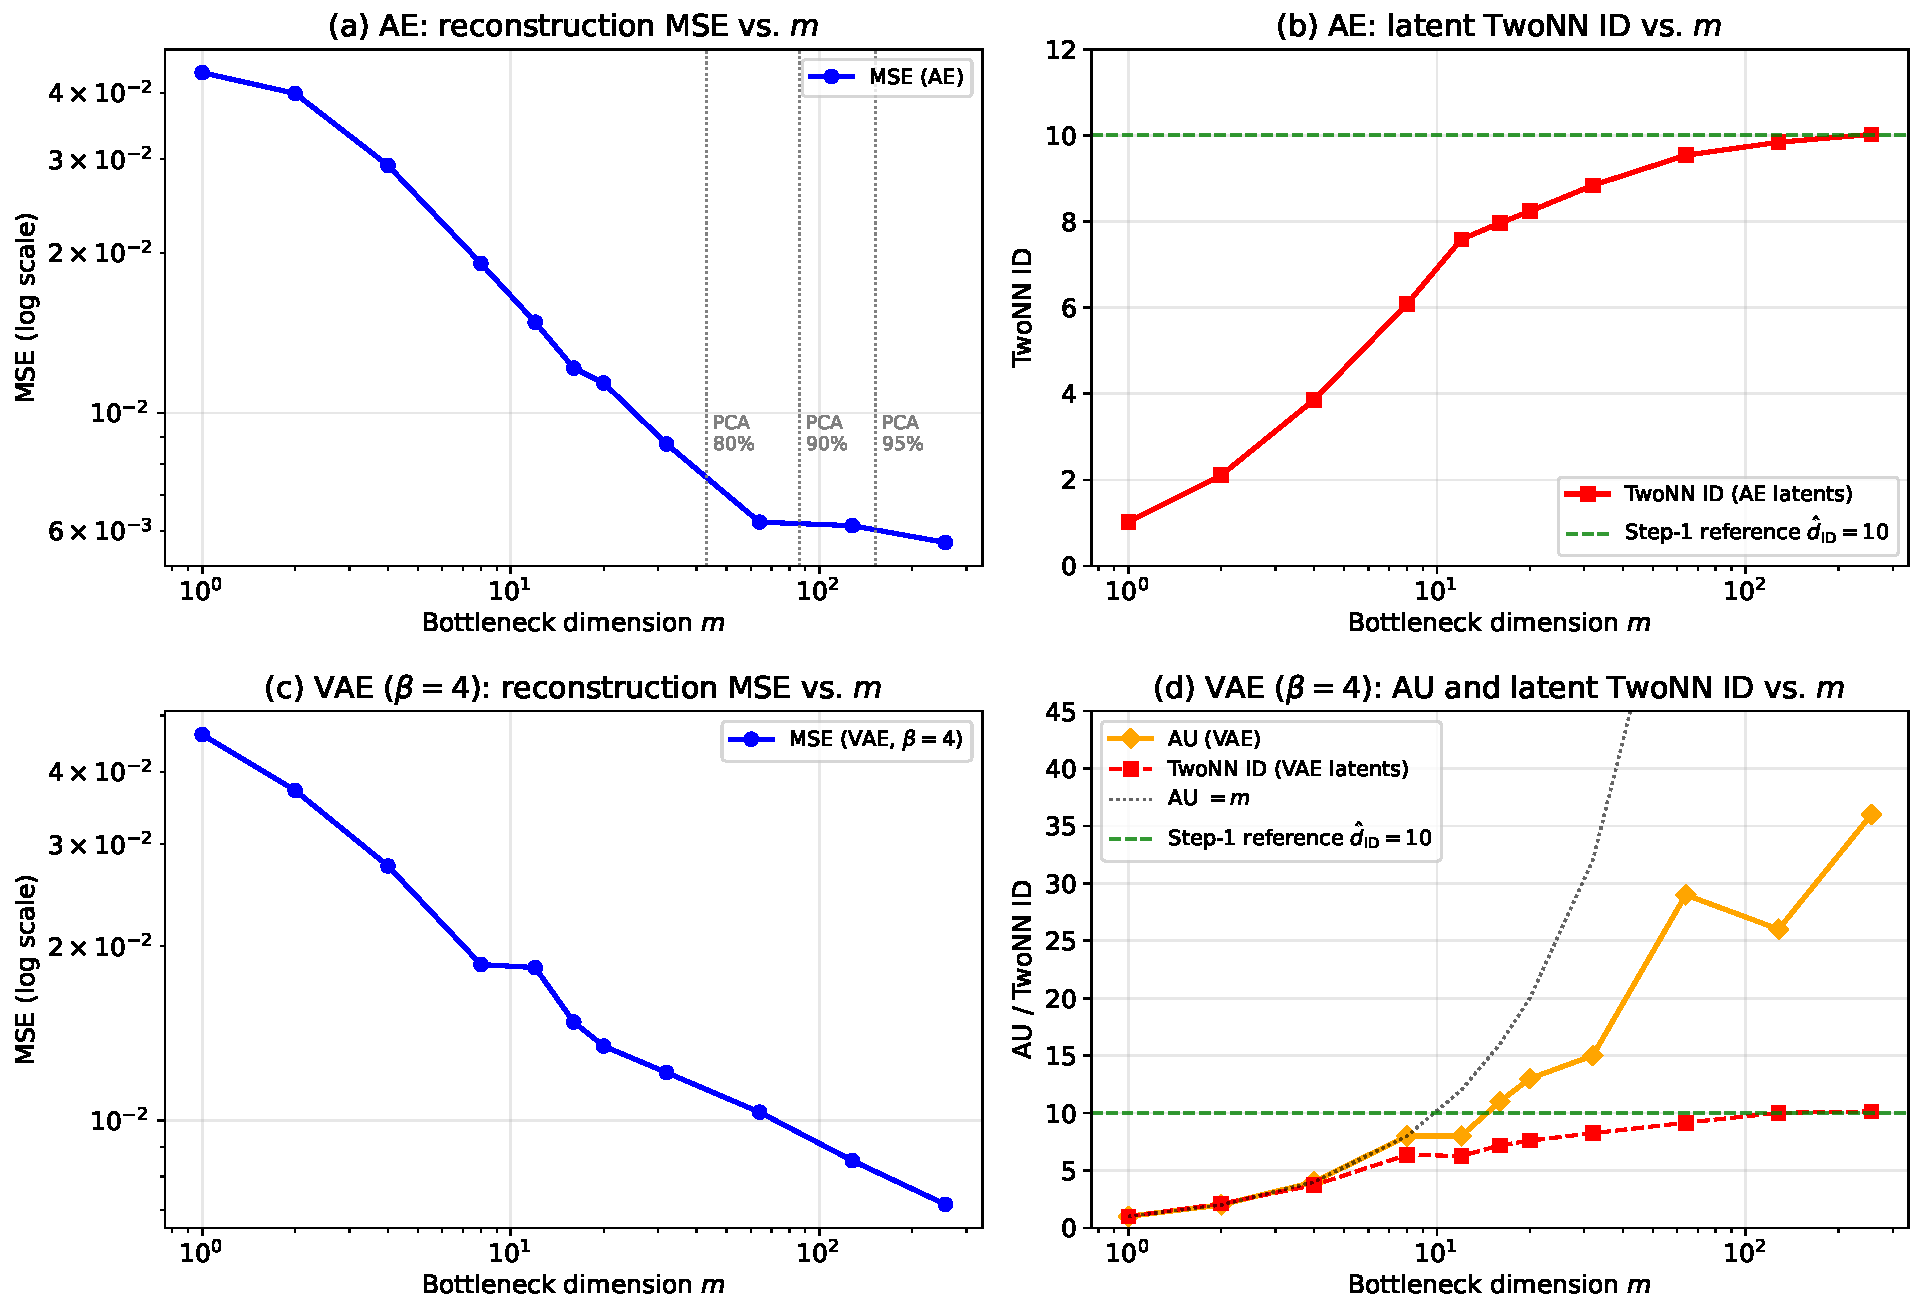
\includegraphics[width=0.95\linewidth]{results/figures/E4_mnist_dualaxis_v43.pdf}
\caption{MNIST: $m$-dependence of the indicators (300 epochs; single-seed
(42) sweep for both the AE and VAE panels---the multi-seed reproducibility
of the VAE AU signal is shown separately in
Figure~\ref{fig:e4_multiseed}).
The single-seed VAE sweep is included for visualizing the dependence on
$m$; all principal VAE verification decisions are based on the independent
three-seed results in Table~\ref{tab:mnist_s3} and
Figure~\ref{fig:e4_multiseed}.
\textbf{(a)} AE reconstruction MSE (log scale); vertical dotted lines mark
the PCA 80/90/95\% cumulative-variance dimensions (43/86/152), far above
the nonlinear estimate $\hatdID \approx 10$.
\textbf{(b)} TwoNN ID on the AE latents.
\textbf{(c)} VAE ($\beta = 4$) reconstruction MSE.
\textbf{(d)} VAE AU and latent TwoNN ID; the AU growth slows beyond
$m \approx \hatdID$ (the vertical axis is clipped at 45 for readability, so
the dotted AU $= m$ diagonal leaves the plotted range).
In panels (b) and (d), the dashed horizontal line marks the rounded Step-1
TwoNN reference $\hatdID = 10$---an estimator-derived reference value, not
a ground-truth dimension.}
\label{fig:e4_dualaxis}
\end{figure}}{}

\IfFileExists{results/figures/E4_300ep_multiseed_v43.pdf}{%
\begin{figure}[H]
\centering
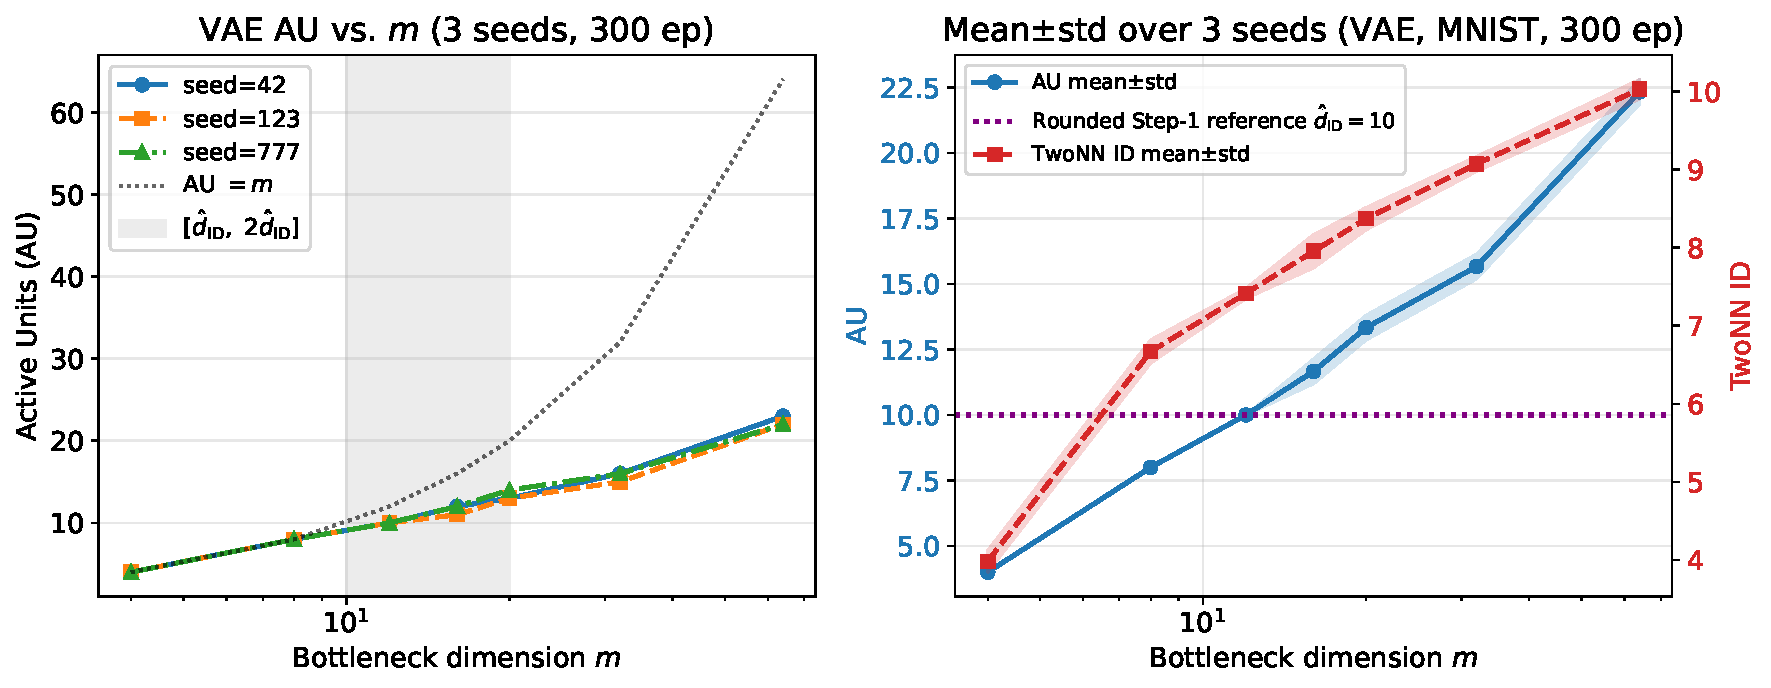
\includegraphics[width=0.9\linewidth]{results/figures/E4_300ep_multiseed_v43.pdf}
\caption{MNIST: multi-seed reproducibility of the AU verification signal
(3 seeds, 300 epochs). Left: per-seed AU$(m)$ with the ID-guided search
window $[\hatdID, 2\hatdID]$ shaded; right: mean$\pm$std band with the
rounded Step-1 TwoNN reference $\hatdID = 10$ (an estimator-derived
reference value, not a ground-truth dimension). AU values are highly
reproducible ($\sigma \leq 0.5$). Change-point (knee) estimates are
deliberately not shown here; they are exploratory only
(Appendix~\ref{app:knee}).}
\label{fig:e4_multiseed}
\end{figure}}{}

\subsubsection{Fine-Grained View of the Slowdown Region and a Caution on Change-Point Detection}\label{sec:exp_mnist_dense}

To inspect the onset of the slowdown more closely, we observed the AU curve
on a dense grid with unit steps around $\hatdID$,
$m \in \{8, 9, \ldots, 16, 18, 20, 24, 28, 32, 40, 48, 64\}$ (17 points,
300 epochs, 3 seeds).
AU$(m)$ stays on the diagonal (AU $= m$) up to $m = 8$--10 and departs from
it at $m \geq 11$; applying a change-point detector based on
first-difference ratios (threshold $\tau_{\mathrm{knee}} = 0.25$;
Appendix~\ref{app:knee}) to this dense grid gives a change point of
$10.3 \pm 0.9$ (per seed: 11, 9, 11), consistent with
$\hatdID \approx 10$.

This agreement, however, carries two important qualifications.
First, the dense-grid region was placed around the Step-1 TwoNN estimate,
so the result is a \textbf{local curve summary conditional on a
TwoNN-derived search window}, not an independent cross-validation.
Second, applying the same detector to the sparse grid
$\{4, 8, 12, 16, 20, 32, 64\}$ yields a change point of $43 \pm 15$---%
\textbf{automatic change-point detection depends strongly on grid design and
should not be operated as a named output of the protocol}.
For this reason, Step 3 relies primarily on the robust read-out
(multi-seed comparison of the AU values themselves---whether the slowdown
region is of the same order as $\hatdID$), and change-point detection is
used only as an aid for grid design (detailed sensitivity analysis in
Appendix~\ref{app:knee}).

\subsubsection{Fashion-MNIST}\label{sec:exp_fashion}

For Fashion-MNIST, Exp-Real-Geom (Section~\ref{sec:exp_real_geom}; 3 seeds,
300 epochs) gives $\hatdID \approx 10$: TwoNN converges to $9.9$--$10.1$
at $m_{\mathrm{ref}} = 5d$--$10d$, where $d = 9$ is the sweep-grid design
value taken from the preliminary 100-epoch estimate
(Appendix~\ref{app:exploratory}).
Step 2 then gives the verification point $m_{\mathrm{ver}} = 2\hatdID = 20$.
Step 3 was run as a 3-seed verification under the same protocol as MNIST
(Exp-Fashion-MS; FC-VAE, $\beta = 4$, 300 epochs,
$m \in \{4, 8, 12, 16, 20, 32, 64\}$; Table~\ref{tab:fashion_s3}).

The result is a \textbf{boundary case} that demonstrates the diagnostic
capability of the decision rule:
all three tested seeds yielded AU $= 7$ at $m = 20$
(AU$(20) = 7.0 \pm 0.0$), so
\textbf{V1 passes} (activation ratio $0.35 \leq 0.9$; truncation operates
robustly) while \textbf{the lower V2 bound is violated}
(AU $= 7 < \hatdID = 10$; all three tested seeds received the same
operational verdict).
Following the diagnosis in the third row of Table~\ref{tab:failure}, this
suggests either that ``$\beta = 4$ sits on the over-regularizing side for
this data--decoder pair'' or that ``the AE-based Step-1 reference includes
variance directions (texture- and style-like factors) that the VAE prunes
at this $\beta$.''
Indeed, the MSE slowdown also occurs at $m \approx 12$--16
(Table~\ref{tab:fashion_s3}), and the preliminary observation that the AU
slowdown region (7--12) is of the same order as $\hatdID$
(Appendix~\ref{app:exploratory}) is itself replicated over the 3 seeds.
Fashion-MNIST is therefore not an example of the protocol mechanically
returning a pass, but a real-data instance in which \textbf{the
pre-registered decision rule detects a boundary case and routes it to the
diagnosis of Table~\ref{tab:failure}}.

\begin{table}[H]
\caption{Exp-Fashion-MS (Fashion-MNIST FC-VAE, $\beta = 4$, 300 epochs,
mean$\pm$std, 3 seeds). At the pre-specified verification point
$m_{\mathrm{ver}} = 20$, V1 passes (activation ratio $0.35$) while the
lower V2 bound is violated (AU $= 7.0 < \hatdID = 10$), with all three
tested seeds receiving the same operational verdict---a diagnostic boundary
case (third row of Table~\ref{tab:failure}).}
\label{tab:fashion_s3}
\small
\begin{tabular}{rccc}
\toprule
$m$ & \textbf{AU} & \textbf{TwoNN ID (latent)} & \textbf{MSE} \\
\midrule
 4 & $4.0 \pm 0.0$ & $3.71 \pm 0.10$ & 0.0184 \\
 8 & $6.3 \pm 0.5$ & $5.44 \pm 0.19$ & 0.0152 \\
12 & $7.0 \pm 0.0$ & $5.90 \pm 0.07$ & 0.0144 \\
16 & $7.3 \pm 0.5$ & $6.10 \pm 0.43$ & 0.0141 \\
\textbf{20} & $\boldsymbol{7.0 \pm 0.0}$ & $5.83 \pm 0.17$ & 0.0143 \\
32 & $9.3 \pm 0.5$ & $6.88 \pm 0.22$ & 0.0130 \\
64 & $11.7 \pm 0.5$ & $7.79 \pm 0.06$ & 0.0120 \\
\bottomrule
\end{tabular}
\end{table}

\subsection{Baseline Comparison: Search Cost and Downstream Performance}\label{sec:exp_downstream}

We quantify the practical value of ID-guided selection against a
\textbf{full $m$-grid search} (Exp-Downstream).
The evaluation metrics are the test classification accuracy of a linear
probe (multiclass logistic regression) on the latent representations and the
reconstruction MSE.

\textbf{AE (reuse of the reference-AE sweep, 300 epochs, seed 42)}:
as shown in the left half of Table~\ref{tab:downstream},
the linear-probe accuracy plateaus at $m = 8$--12 ($92.3\%$ at $m = 12$)
and does not improve up to $m = 256$ ($91.8\%$; raw 784-dimensional pixels:
$91.6\%$).
\textbf{The best observed accuracy over the full grid (11 points),
$92.3\%$, lies inside the ID-guided search window $[10, 24]$ (at
$m = 12$)},
and the other in-range points ($m = 16, 20$) are within 1.4 points of it.

\textbf{VAE ($\beta = 4$, 300 epochs, 3 seeds)}:
as shown in the right half of Table~\ref{tab:downstream}, the same picture
holds on the VAE side: the linear-probe accuracy attains its best observed
mean value over the grid $\{4, \ldots, 64\}$, $89.1 \pm 0.4\%$, at $m = 12$
inside the search window, and is nearly flat for $m \geq 12$.
At the VAE-path verification point $m = 20 = 2\hatdID$ it is
$88.2 \pm 0.4\%$---within $0.9$ percentage points of the best observed mean
accuracy, although the three-seed sample is too small to support a formal
equivalence claim.
The AU and MSE values in this table are retrained reproductions of
Table~\ref{tab:mnist_s3} (Exp-Mnist-Multi-300) and agree with it---an
additional reproducibility check.

\textbf{Search cost}: the full MNIST grid of this paper requires 11 values
of $m$ $\times$ 3 seeds $= 33$ runs.
The ID-guided path instead performs Step 1 (convergence check over
$m_{\mathrm{ref}} \in \{64, 128, 256\}$; 3 single-seed runs) and then either
(a) the AE path: training the in-range grid points $\{12, 16, 20\}$ over 3
seeds (9 runs)---12 runs in total (\textbf{$\approx$64\% saved}); or
(b) the VAE path: training the single point $m = 2\hatdID = 20$ over 3 seeds
and verifying by AU (3 runs)---6 runs in total
(\textbf{$\approx$82\% saved}).
Under the conservative variant that also verifies at the MLE-shifted point
$m = 32$ (Section~\ref{sec:protocol_s3}), the VAE path is 9 runs in total
($\approx$73\% saved).
Note that this accounting counts Step 1 as single-seed runs (this paper
quantifies Step-1 uncertainty separately via subsampling CIs and estimator
cross-checks); a symmetric accounting that repeats Step 1 over 3 seeds
gives 18 runs for the AE path ($\approx$45\% saved) and 12 runs for the VAE
path ($\approx$64\% saved).
Table~\ref{tab:cost} organizes this accounting by condition.
The reduction rates compare \textbf{numbers of training runs only}; they do
not include GPU time, estimator computation, or analysis time.
The retained performance is the descriptive comparison given above (the
best observed accuracy lies inside the window; the VAE verification point
is within $0.9$ points of it).
This comparison is limited to the MNIST grid configuration and linear probe
of this paper and does not establish a general reduction rate
(Section~\ref{sec:disc_model_selection}).

\begin{table}[H]
\caption{Training-run accounting for the specific MNIST grid, epoch count,
seed design, and verification procedure used in this study. ``Runs''
counts model trainings only (Step-1 reference-AE trainings included); GPU
time, estimator computation, and analysis time are not included.}
\label{tab:cost}
\small
\begin{tabular}{lrrrr}
\toprule
\textbf{Path} & \textbf{Full-grid runs} & \textbf{ID-guided runs} & \textbf{Step-1 seeds} & \textbf{Reduction} \\
\midrule
AE, single-seed Step 1 & 33 & 12 & 1 & 64\% \\
VAE, single-seed Step 1 & 33 & 6 & 1 & 82\% \\
VAE + MLE-shifted verification & 33 & 9 & 1 & 73\% \\
AE, three-seed Step 1 & 33 & 18 & 3 & 45\% \\
VAE, three-seed Step 1 & 33 & 12 & 3 & 64\% \\
\bottomrule
\end{tabular}
\end{table}

\begin{table}[H]
\caption{Exp-Downstream (MNIST): linear-probe test accuracy and MSE vs.\
$m$. Left: AE latents (300 epochs, single seed 42; reuse of the
reference-AE sweep). Right: FC-VAE ($\beta = 4$) latents (300 epochs,
mean$\pm$std, 3 seeds). Bold $m$ values lie in the ID-guided search window
$[10, 24]$, which contains the best observed accuracy over the full grid;
for the VAE, $m = 20$ is in addition the pre-specified verification point
$m_{\mathrm{ver}}$ (Section~\ref{sec:protocol_s3}).
Raw-pixel baseline: $91.6\%$.
Because the AE results are based on a single reference-AE seed, the AE
probe accuracies should be interpreted descriptively rather than as
multi-seed performance estimates.}
\label{tab:downstream}
\small
\begin{tabular}{r cc | r ccc}
\toprule
\multicolumn{3}{c|}{\textbf{AE (single seed)}} & \multicolumn{4}{c}{\textbf{VAE ($\beta = 4$, 3 seeds)}} \\
$m$ & Probe acc.\ (\%) & MSE & $m$ & Probe acc.\ (\%) & AU & MSE \\
\midrule
1 & 60.0 & 0.0437 & 4 & $85.0 \pm 0.5$ & $4.0 \pm 0.0$ & 0.0282 \\
2 & 60.0 & 0.0399 & 8 & $87.7 \pm 0.1$ & $8.0 \pm 0.0$ & 0.0182 \\
4 & 81.7 & 0.0292 & \textbf{12} & $\boldsymbol{89.1 \pm 0.4}$ & $10.0 \pm 0.0$ & 0.0154 \\
8 & 91.7 & 0.0191 & \textbf{16} & $89.0 \pm 0.2$ & $11.7 \pm 0.5$ & 0.0138 \\
\textbf{12} & \textbf{92.3} & 0.0148 & \textbf{20} & $88.2 \pm 0.4$ & $13.3 \pm 0.5$ & 0.0126 \\
\textbf{16} & 92.0 & 0.0121 & 32 & $88.1 \pm 0.2$ & $15.7 \pm 0.5$ & 0.0112 \\
\textbf{20} & 90.9 & 0.0114 & 64 & $88.7 \pm 0.3$ & $22.3 \pm 0.5$ & 0.0089 \\
32 & 91.2 & 0.0087 &  & & & \\
64 & 91.8 & 0.0062 &  & & & \\
128 & 92.2 & 0.0061 &  & & & \\
256 & 91.8 & 0.0057 &  & & & \\
\bottomrule
\end{tabular}
\end{table}

\subsection{Validity Condition of Step 1: What Makes Intrinsic-Dimension Estimation Stable?}\label{sec:exp_real_geom}

Since Step 1 goes through the latents of a reference AE, the focus is
whether the geometric distortion of the reference representation corrupts
the estimate.
In Exp-Real-Geom we swept four models with different isometry properties
(plain AE / IsometricAE~\cite{kato2020rdae} / CAE~\cite{rifai2011cae} /
DAE~\cite{alain2014dae}) on MNIST and Fashion-MNIST over
$m_{\mathrm{ref}} \in \{d, 2d, 3d, 5d, 10d\}$
($d$ is the grid design value from preliminary estimates: 10 for MNIST,
9 for Fashion-MNIST), comparing TwoNN, MLE,
$\kap$, Trustworthiness, and kNN overlap (3 seeds, 300 epochs).

\begin{table}[H]
\caption{Exp-Real-Geom (MNIST, mean$\pm$std, 3 seeds): TwoNN through four
reference models. Convergence is driven by the bottleneck margin
$m_{\mathrm{ref}} / \hatdID$, largely independently of the isometry
(condition number $\kap$).}
\label{tab:real_geom}
\footnotesize
\begin{tabular}{lcccc}
\toprule
\textbf{Model} & \textbf{TwoNN ($m_{\mathrm{ref}} = d$)} & \textbf{TwoNN ($m_{\mathrm{ref}} = 5d$)} & \textbf{TwoNN ($m_{\mathrm{ref}} = 10d$)} & $\kap$ \textbf{($m_{\mathrm{ref}} = 10d$)} \\
\midrule
AE          & $7.3 \pm 0.4$ & $10.0 \pm 0.1$ & $10.0 \pm 0.1$ & $4.1 \times 10^{7}$ \\
IsometricAE & $7.5 \pm 0.4$ & $10.1 \pm 0.1$ & $10.1 \pm 0.1$ & $7.8$ \\
CAE         & $7.2 \pm 0.5$ & $9.9 \pm 0.1$  & $10.0 \pm 0.1$ & $3.2 \times 10^{3}$ \\
DAE         & $7.6 \pm 0.4$ & $10.0 \pm 0.1$ & $10.0 \pm 0.1$ & $6.3 \times 10^{3}$ \\
\bottomrule
\end{tabular}
\end{table}

The results (Table~\ref{tab:real_geom}) are clear:
(1) in all four models, TwoNN converges from the underestimate at
$m_{\mathrm{ref}} = d$ ($\approx 7.3$--7.6) to $\approx 10$ at
$m_{\mathrm{ref}} \geq 5d$, and the inter-model differences (within
$\pm 0.3$) are an order of magnitude smaller than the effect of increasing
$m_{\mathrm{ref}}$ (about 2.5 points);
(2) IsometricAE improves $\kap$ from $10^{7}$ to around $8$, yet its effect
on TwoNN stays within $\pm 0.2$.
The same pattern was obtained on Fashion-MNIST.
That is, \textbf{under the datasets, architectures, sample sizes, and
estimators tested here, the dominant condition for Step-1 stability is not
``improved isometry'' but the ``bottleneck margin
$m_{\mathrm{ref}} \gg \hatdID$''} (consistent with the $\delta_T$-dominance
implication of the conditional-stability rationale in
Section~\ref{sec:theory_twonn}), justifying the design
of Step 1 with a plain reference AE at $m_{\mathrm{ref}} = 256 \gg \hatdID$
(Figure~\ref{fig:ep}).

\IfFileExists{results/figures/EP_twonn_stability.pdf}{%
\begin{figure}[H]
\centering
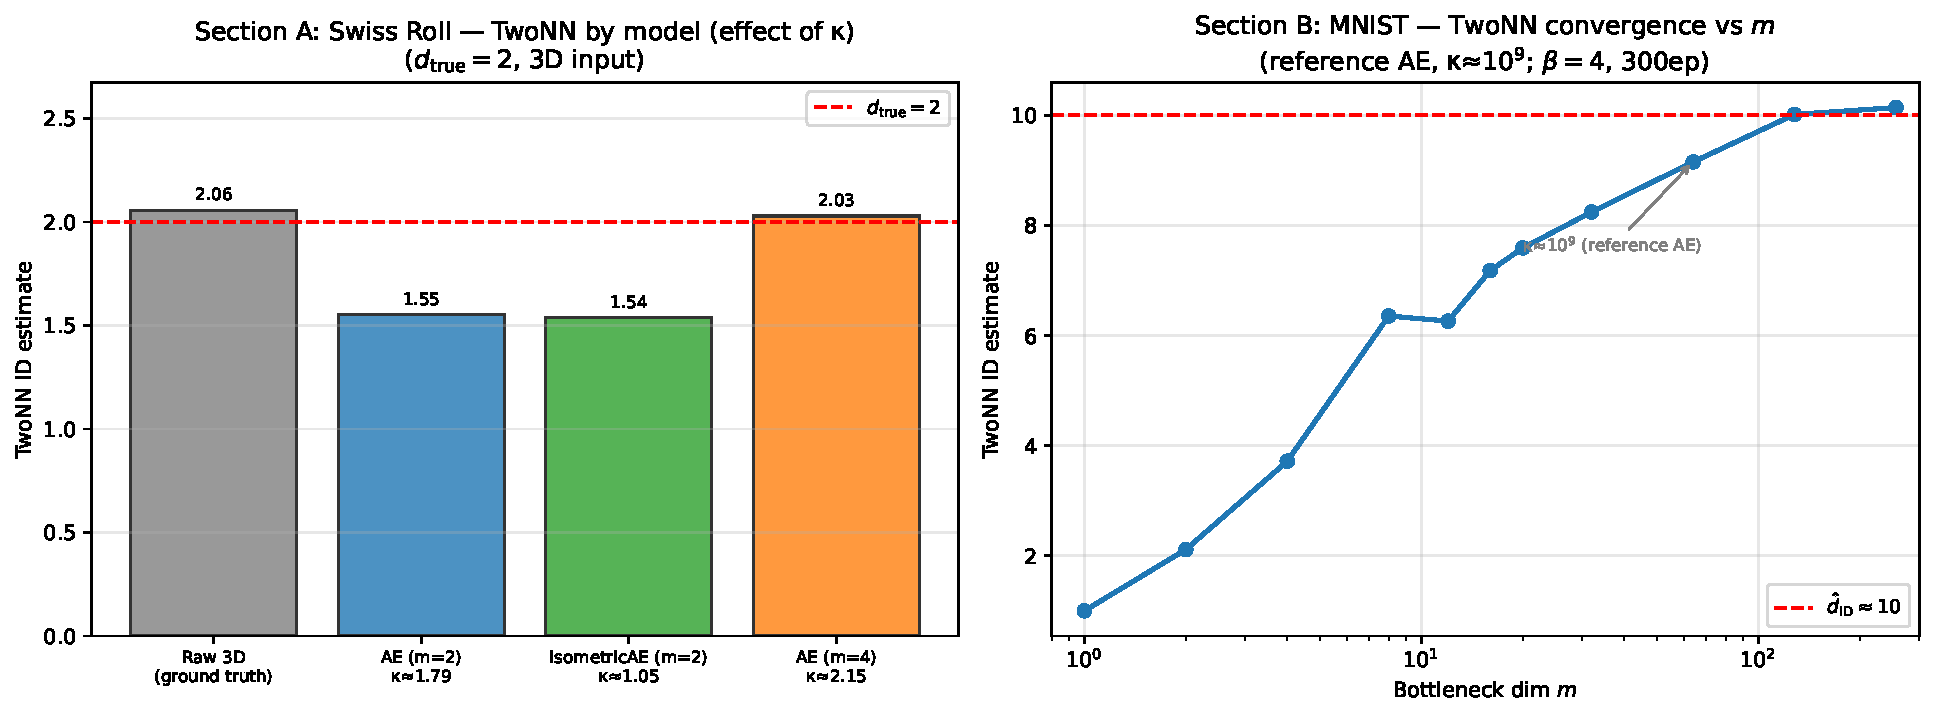
\includegraphics[width=0.95\linewidth]{results/figures/EP_twonn_stability.pdf}
\caption{Step-1 stability: (left) on the Swiss Roll, TwoNN recovers once
$m_{\mathrm{ref}} > \dtrue$ across the tested reference models, despite
large differences in the decoder-Jacobian condition number; (right) on
MNIST, TwoNN stabilizes for $m_{\mathrm{ref}} \geq 48 \approx 5\hatdID$
even where the condition number $\kap$ grows sharply.
This result does not establish that isometry is generally irrelevant to
intrinsic-dimension estimation.}
\label{fig:ep}
\end{figure}}{}

\subsection{Applicability Boundary: Conv-VAEs and Natural Images}\label{sec:exp_boundary}

This section is not a ``report of failures'' of the protocol but a
quantification of the conditions under which the failure modes of
Table~\ref{tab:failure} actually occur.

\subsubsection{Conv-VAE: Truncation Failure Due to Insufficient $\beta$ (3 Seeds)}

We swept an MNIST Conv-VAE (2 Conv layers + 2 ConvTranspose layers, KL
cyclic annealing with $\beta_{\max} = 4$~\cite{fu2019cyclical}, 150 epochs,
3 seeds) over $m \in \{4, 8, 16, 32, 64, 96, 128, 192, 256\}$
(Exp-Conv-M256).
For $m \leq 64$, AU $= m$ (no truncation) persists in all seeds; AU falls
below $m$ for the first time at $m = 96$ (AU $= 90.7 \pm 1.2$), yet the
activation rate remains as high as 94\% at $m = 256$
(Figure~\ref{fig:en}).
Extending to $m \in \{384, 512\}$ (Exp-Conv-M512) still keeps
AU $\approx m$---that is, at $\beta_{\max} = 4$ the experiments do not
observe substantial truncation within $m \leq 512$; under the surrogate
interpretation, this pattern is consistent with an effective truncation
threshold beyond the tested range
($d^*_{\mathrm{eff}}(\beta) > 512$)---and \textbf{the AU verification
detects the state
``$\beta$ too small relative to the decoder capacity'' through the clear
signal AU $= m$} (first row of Table~\ref{tab:failure}).

Two caveats frame the surrogate-based interpretation below.
First, the surrogate analysis of Proposition~\ref{thm:linear_vae} assumes
a \textbf{fixed} $\beta$, whereas the convolutional experiments use
cyclical KL annealing (three cycles; within each cycle, $\beta$ increases
linearly from $0$ to $\beta_{\max}$ over the first half and is held at
$\beta_{\max}$ over the second half~\cite{fu2019cyclical});
$\beta_{\max}$ is therefore a training-schedule parameter and should not
be identified with the fixed $\beta$ appearing in
Proposition~\ref{thm:linear_vae}.
Second, the discussion of $\tau^2_{\mathrm{eff}}$ below is a post-hoc
heuristic interpretation intended to connect the observed behavior with
the linear surrogate; it is not an independently estimated physical or
probabilistic parameter of the nonlinear decoder.
From the viewpoint of the surrogate condition
(Proposition~\ref{thm:linear_vae}), a powerful convolutional decoder makes
the effective noise variance $\tau^2_{\mathrm{eff}}$ small (a back-computed
calibration $\approx 0.30$ for the FC-VAE and $\ll 0.30$ for the Conv-VAE; a
heuristic extrapolation), lowering the threshold
$\beta\tau^2_{\mathrm{eff}}$ and inflating $\dstar$.
This interpretation is consistent with the $\beta$-strengthening
experiments: at $\beta_{\max} = 10$, AU $= 95.7 \pm 5.2$ (activation ratio
37\%) at $m = 256$; at $\beta_{\max} = 20$, AU $= 68.0 \pm 2.2$
(27\%)---a clear reduction in the activation ratio and evidence of stronger
truncation within the tested range, although stable AU saturation (a
plateau in $m$) was not established
(Exp-ConvV-HiBeta; \textbf{3 seeds}, details in
Appendix~\ref{app:exploratory}).
This is consistent with the qualitative prediction that increasing $\beta$
moves the truncation to lower dimensions, identifying ``strengthening
$\beta$ according to data and architecture'' as a necessary condition for
applying the protocol to Conv-VAEs.

\textbf{Verdict} (MNIST Conv-VAE):
Step 1---usable (reusing $\hatdID \approx 10$ from the FC reference AE);
Step 2---search window obtained ($m \geq 20$);
Step 3---\textbf{fail} at $\beta_{\max} = 4$ (activation ratio
$0.94 > 0.9$ at $m = 256$; V1 violated).
At $\beta_{\max} \in \{10, 20\}$, V1 holds (activation ratios $0.37$ and
$0.27$; all three tested seeds received the same operational verdict) but V2
remains violated since AU $= 95.7 \pm 5.2$ and
$68.0 \pm 2.2 > 3\hatdID = 30$;
we judge this as ``truncation induced, but order consistency with $\hatdID$
not yet achieved.''

\IfFileExists{results/figures/EN_conv_vae_extended_m_v44.pdf}{%
\begin{figure}[H]
\centering
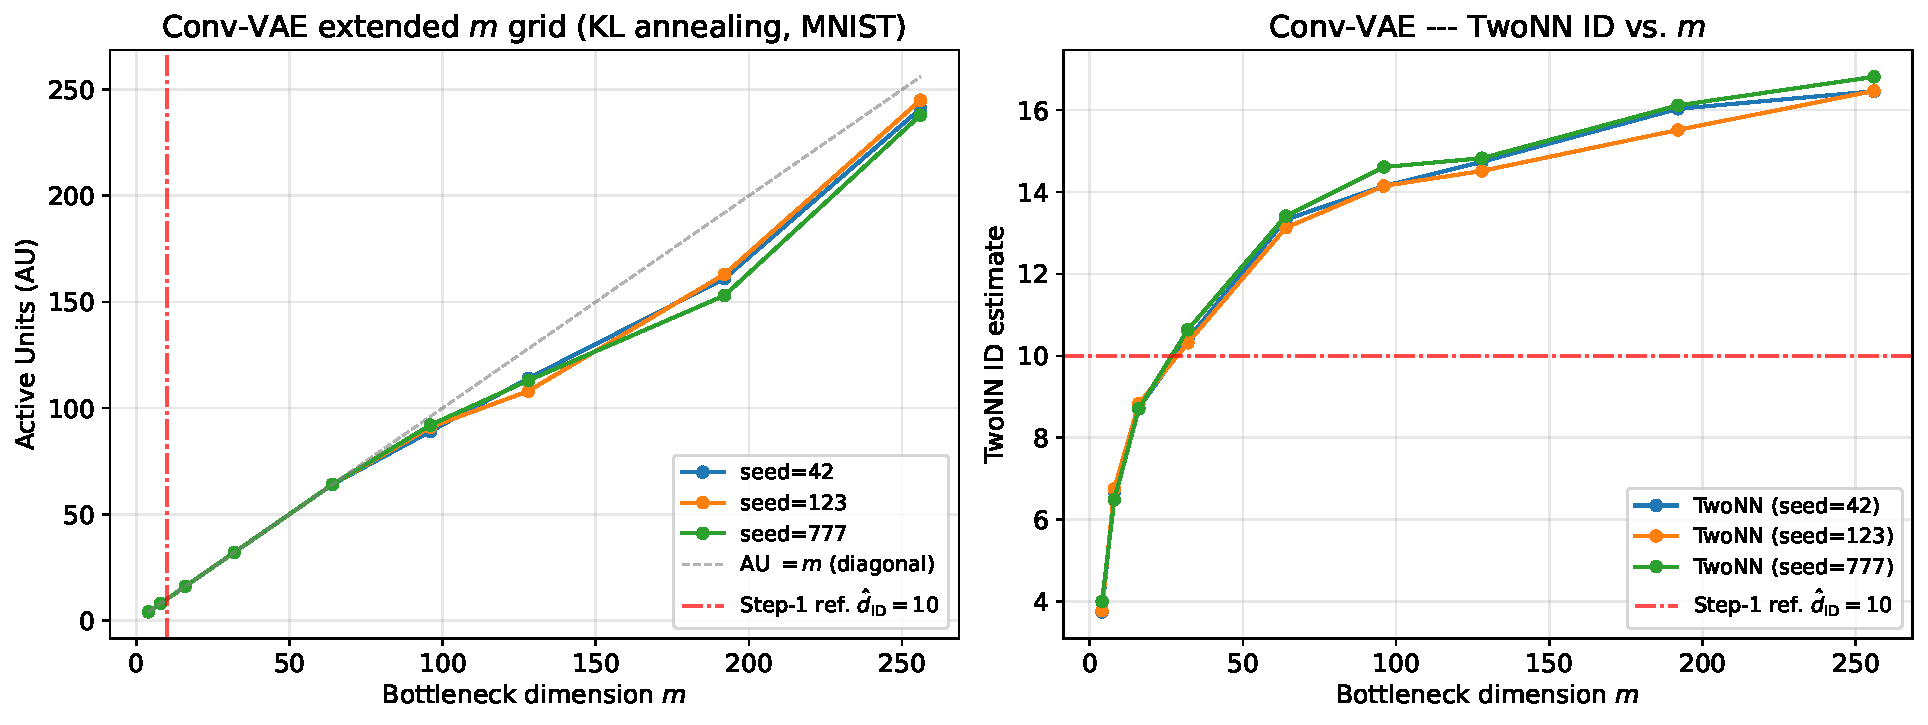
\includegraphics[width=0.95\linewidth]{results/figures/EN_conv_vae_extended_m_v44.pdf}
\caption{Boundary condition (Exp-Conv-M256): the MNIST Conv-VAE with
$\beta_{\max} = 4$ keeps AU $= m$ (no truncation) up to $m = 64$ and stays
at 94\% activation even at $m = 256$---the failure mode ``$\beta$ too small
relative to decoder power'' detected by the AU signal.
The reference value $\hatdID = 10$ was obtained from the independently
trained reference-AE procedure of Step 1, not from the Conv-VAE latents
shown here.}
\label{fig:en}
\end{figure}}{}

\subsubsection{Natural Images: Bounded Trust Region of Step 1 and Unmet Step 3 (3 Seeds)}

For Conv-VAEs on CIFAR-10~\cite{krizhevsky2009learning} and
SVHN~\cite{netzer2011reading} (3 Conv layers, $\beta_{\max} = 4$,
150 epochs, 3 seeds, $m \in \{16, 32, 64, 128, 256\}$), two observations
follow (Table~\ref{tab:natural}).
First, \textbf{Step 1 works conditionally}: the latent TwoNN of CIFAR-10 at
$m = 64 \approx 2\hatdID$ is $25.21 \pm 0.41$, consistent with the raw-input
estimate (25.20) and with Pope et al.~\cite{pope2021intrinsic}
($\approx 26$).
Beyond $m \geq 128$, however, it inflates monotonically to
$28.8$--$30.9$---\textbf{on natural images the estimate is consistent with
prior estimates only near $m_{\mathrm{ref}} \approx 2\hatdID$, and ``the
larger the better'' does not hold} (the true ID is unknown, so nothing
stronger than consistency can be claimed; fourth failure mode of
Table~\ref{tab:failure}).
For the natural-image experiments considered here,
$m_{\mathrm{ref}} \approx 2\hatdID$ thus behaved as a \textbf{provisional
consistency region}, not as a validated selection rule.
The contrast with MNIST (stable even at $m_{\mathrm{ref}} = 25\hatdID$) is
attributed to latent-geometry distortion while all dimensions remain in use
(AU $= m$, no truncation).
For SVHN the discrepancy is even larger (latent 27.1 vs.\ raw 10.1 at
$m = 256$).
This discrepancy should not by itself be interpreted as latent-space
inflation: the raw-input estimate is not a ground truth either, as it may
be affected by ambient-dimensional distance concentration and by
heterogeneous local geometry (Section~\ref{sec:related}), so the two
values are best read as two differently biased views of an unknown
quantity.

\textbf{Why is the distortion so pronounced on natural images
(hypotheses)?}
We regard the gap between MNIST and natural images not as a matter of
degree but as reflecting a qualitative difference in data geometry.
\textbf{The following mechanisms are hypotheses consistent with the
observed pattern, not experimentally distinguished explanations.}
First, \textbf{manifold entanglement}---operationally, a distribution
structured as a union of submanifolds whose local intrinsic dimension
varies strongly across classes and regions, in conflict with the
single-global-metric assumption of TwoNN: MNIST consists of centered,
size-normalized single objects whose dominant factor is smooth stroke
deformation, and is therefore well approximated by a single smooth
manifold; natural images are compositions of factors at different
scales---object category, pose, texture, lighting, background---and behave
like such a union of submanifolds (Pope et
al.~\cite{pope2021intrinsic} likewise report large inter-class variation
of the ID, and Allegra et al.~\cite{allegra2020data} provide a related
treatment of heterogeneous local intrinsic dimensionality).
For TwoNN, which assumes a single global metric, such inhomogeneous
structure tends to degrade the preservation of neighbor ranks (the
$\delta_T$ of Section~\ref{sec:theory_twonn}) as $m_{\mathrm{ref}}$
grows.
Second, \textbf{high-frequency texture and the effective noise variance}:
reconstructing natural images requires encoding fine texture, and a
powerful Conv decoder drives $\tau^2_{\mathrm{eff}}$ extremely small.
As a result $\dstar \gg m$ and truncation vanishes; in a latent space where
all coordinates remain in use, the dominant manifold factors and the
texture residuals are mixed within one metric and the neighborhood
structure is distorted---consistent with the pattern observed in our
experiments, where AU $= m$ and TwoNN inflation occur simultaneously.
Third, \textbf{the need for hierarchical latent structure}: generative
factors of natural images form a scale hierarchy from global (objects) to
local (texture), and the architectural mismatch of forcing this hierarchy
into a single flat latent vector with an isotropic prior may itself be a
source of distortion.
Under this hypothesis, a natural next step is to apply the protocol
per level to the scale-wise latents of hierarchical
VAEs~\cite{sonderby2016ladder} (reading the AU of each level separately)
(Section~\ref{sec:disc_limitation}).
All three hypotheses are consistent with our observations (persistent
AU $= m$, $m_{\mathrm{ref}}$-dependent TwoNN inflation, partial recovery
under $\beta$-strengthening), but a direct disambiguation is left for
future work.
Second, \textbf{Step 3 is unmet}: no AU saturation appears for
$m \leq 256$ (only AU $< m$ from $m \geq 128$ on SVHN); AU verification
requires strengthened $\beta$, restricted decoder capacity, and exploration
of larger $m$ ranges (a preliminary observation of plateau-like behavior at
$\beta_{\max} = 80$ with a thin decoder is reported in
Appendix~\ref{app:exploratory}).

\textbf{Verdict} (natural images):
Step 1---usable only in the provisional consistency region
$m_{\mathrm{ref}} \approx 2\hatdID$
(CIFAR-10: $25.21 \pm 0.41$, consistent with reported values; inflation
beyond);
Step 2---search window obtained conditionally (CIFAR-10: $m \geq 50$);
Step 3---\textbf{unresolved} (CIFAR-10: activation ratio $1.0$ at $m = 256$,
V1 violated; SVHN: activation ratio $0.81$ satisfies V1 but
AU $= 206.7 \gg 3\hatdID$ violates V2).

\begin{table}[H]
\caption{Natural images (Exp-Nat-Cifar / Exp-Nat-SVHN): Conv-VAE with KL
cyclic annealing ($\beta_{\max} = 4$, 150 epochs, mean$\pm$std, 3 seeds).
For CIFAR-10, Step 1 agrees with Pope et al.~\cite{pope2021intrinsic} only
near $m \approx 2\hatdID$ (for SVHN the latent--raw discrepancy is larger;
see text); Step 3 (AU saturation) is not reached in the tested range.}
\label{tab:natural}
\small
\begin{tabular}{r cc | cc}
\toprule
 & \multicolumn{2}{c|}{\textbf{CIFAR-10}} & \multicolumn{2}{c}{\textbf{SVHN}} \\
$m$ & \textbf{AU} & \textbf{TwoNN ID} & \textbf{AU} & \textbf{TwoNN ID} \\
\midrule
 16 & $16.0 \pm 0.0$ & $13.12 \pm 0.12$ & $16.0 \pm 0.0$ & $11.30 \pm 0.12$ \\
 32 & $32.0 \pm 0.0$ & $19.26 \pm 0.23$ & $32.0 \pm 0.0$ & $15.08 \pm 0.08$ \\
 64 & $64.0 \pm 0.0$ & $\mathbf{25.21 \pm 0.41}$ & $64.0 \pm 0.0$ & $19.97 \pm 0.12$ \\
128 & $128.0 \pm 0.0$ & $28.83 \pm 0.41$ & $125.3 \pm 0.5$ & $24.60 \pm 0.36$ \\
256 & $256.0 \pm 0.0$ & $30.91 \pm 0.64$ & $206.7 \pm 1.2$ & $27.08 \pm 0.34$ \\
\midrule
\multicolumn{3}{l|}{Raw-input TwoNN $= 25.20$, MLE $= 26.56$} &
\multicolumn{2}{l}{Raw-input TwoNN $= 10.09$, MLE $= 18.85$} \\
\bottomrule
\end{tabular}
\end{table}

%% ===================================================================
\section{Discussion}\label{sec:discussion}

\subsection{What Differs from Conventional Model-Selection Criteria?}\label{sec:disc_model_selection}

The conventional means of choosing $m$ in practice are $m$-sweeps of
validation reconstruction error or ELBO, or downstream task performance.
These tell us ``the $m$ at which performance plateaus,'' but
(i) they require sweeping the entire grid, and
(ii) they do not distinguish the cause of the plateau (data manifold
dimension, model capacity, or optimization).
Our protocol does not replace them but \textbf{complements} them:
Step 1 narrows the search window to the vicinity of $\hatdID$ before any
sweep (reducing search cost), and the AU of Step 3 reports---independently
of performance---how many dimensions are actually in use, directly
visualizing the presence of redundant dimensions.
Indeed, on MNIST the MSE verification, the AU verification, $\hatdID$, and
the linear-probe accuracy all supported the same search window $[10, 24]$
(Section~\ref{sec:exp_downstream}), and on the MNIST grid used in this
paper, choosing $m$ inside the window reduced the number of training runs
by roughly 60--80\% relative to the full grid search while nearly retaining
the downstream classification accuracy (no general reduction rate is
claimed).
This comparison is, however, limited to a linear probe on MNIST; systematic
comparison with nonlinear downstream tasks and disentanglement metrics
remains future work.

\subsection{Stability vs.\ Validity: What Does $\hatdID$ Estimate?}\label{sec:disc_twonn}

A distinction maintained throughout this paper is that
``TwoNN/MLE being \textbf{numerically stable} (low variance across seeds and
$m_{\mathrm{ref}}$)'' is different from ``being \textbf{unbiased} with
respect to the true intrinsic dimension.''
The latent space of the reference AE is far from isometric ($\kap$ reaches
$10^{7}$; Table~\ref{tab:real_geom}), and what TwoNN estimates is, strictly
speaking, ``the local degrees of freedom of the reference representation.''
The MNIST value $\hatdID \approx 10$--12 is supported by several pieces of
indirect evidence---(i) convergence over multiple $m_{\mathrm{ref}}$,
(ii) TwoNN--MLE agreement, (iii) agreement across four reference models
(Table~\ref{tab:real_geom}), (iv) narrow subsampling CIs and
order-of-magnitude agreement with estimators of different principles
(DANCo, ESS; Table~\ref{tab:boot_ci}), and (v) consistency with reported
values on CIFAR-10---but this is not a direct proof of unbiasedness.
The protocol therefore operates $\hatdID$ as ``a reference value giving the
center of the search window'' and closes the loop with the Step-3
verification.
A remaining task is the calibration of $\hatdID$ against ground truth beyond
synthetic data (a systematic evaluation of estimator bias).

\subsection{Limits of AU Verification: Why Change-Point Detection Is Not a Named Output}\label{sec:disc_knee}

An earlier version of this framework (the predecessor of this work) treated
the AU slowdown point $\mknee$ as one of its diagnostics; this paper removes
it from the named outputs.
The reasons, shown in Section~\ref{sec:exp_mnist_dense}, are that
(i) the sparse-grid detection ($43 \pm 15$) is dominated by the grid
interval,
(ii) stabilization requires a TwoNN-derived search window and hence is not
independent validation, and
(iii) the detection is also sensitive to the choice of detector
(threshold vs.\ second difference) (Appendix~\ref{app:knee}).
The robust part of AU verification is the read-out ``do the AU values
themselves (multi-seed, $\sigma \leq 0.5$) slow down or saturate at the same
order as $\hatdID$?''---the protocol is designed to use only this robust
part in its decision rule
(Equations~\eqref{eq:rule_v1}--\eqref{eq:rule_v2}, which involve no
change-point detection).
Nested validation, in which the search-window estimation and the
change-point evaluation are performed on disjoint seeds or data subsets,
remains future work.

\subsection{Limitations and Future Work}\label{sec:disc_limitation}

\begin{itemize}
  \item \textbf{Validation scope}: multi-seed validation of the full
        protocol is limited to synthetic manifolds and the MNIST and
        Fashion-MNIST AU verifications (the MNIST Step-1 sweep is
        single-seed with separately quantified uncertainty---a full
        multi-seed reference-AE sweep over all $m_{\mathrm{ref}}$ values
        was not performed; the Fashion-MNIST Step 3 is a diagnostic
        detection example with V1 passing and the lower V2 bound violated;
        Section~\ref{sec:exp_fashion}).
        In addition, all experiments use fixed-order data subsets
        (Section~\ref{sec:exp_setup}), so the results are not averages
        over independent data partitions.
        The recovery of Conv-VAE truncation by strengthened $\beta$
        (Exp-ConvV-HiBeta) was replicated over 3 seeds (V1 holds, V2
        unmet; Section~\ref{sec:exp_boundary}), but achieving order
        consistency requires joint control of $\beta$ and decoder
        capacity.
  \item \textbf{Step 3 on natural images}: stable identification of AU
        saturation is unmet; dense sweeps of
        $\beta_{\max} \in [40, 120]$, decoder-capacity control, and improved
        seed stability are future work (Appendix~\ref{app:exploratory}).
        The hypotheses stated in Section~\ref{sec:exp_boundary} (manifold
        entanglement, texture-driven shrinkage of $\tau^2_{\mathrm{eff}}$,
        and the need for hierarchical latent structure) also suggest
        directions for improvement:
        (i) applying the protocol per level to the scale-wise latents of
        hierarchical VAEs~\cite{sonderby2016ladder}, reading the AU
        truncation at the level of global factors;
        (ii) class-conditional or region-wise estimation of $\hatdID$ per
        submanifold (mitigating the inhomogeneity of the union structure);
        (iii) bounding $\tau^2_{\mathrm{eff}}$ from below via decoder
        capacity or rate-allocation control (separating texture residuals
        from the AU diagnosis).
        These extensions keep the estimate--set--verify framework of the
        protocol itself and refine Steps 1 and 3 to operate per level or
        per subset.
  \item \textbf{$\beta$ dependence and decision thresholds}: the AU
        read-out depends on $\beta$
        (AU patterns confirmed stable for $\beta \in [2, 8]$;
        Appendix~\ref{app:sens}), and AU is coordinate-dependent
        (Section~\ref{sec:protocol_setup}), so its read-out is tied to the
        chosen prior and latent parameterization.
        Actively exploiting the $\beta$ dependence of $\dstar$---a
        ``spectral read-out by $\beta$ sweep''---is an interesting
        extension.
        The thresholds of the decision rule (activation ratio $0.9$, factor
        $3$) are working defaults that separate the passing and failing
        cases of this paper by a wide margin; calibrating them on more
        diverse data is future work.
  \item \textbf{Scope of the theory}: Proposition~\ref{thm:linear_vae} is a
        linear-Gaussian approximation, and its nonlinear extrapolation rests
        on post-hoc consistency checks via $\tau^2_{\mathrm{eff}}$.
        Deriving activation conditions in nonlinear settings is open.
  \item \textbf{Computational cost}: the multi-seed $m$-sweep of Step 3
        takes hours to a day of GPU time.
        Step 1 shrinks the sweep range, but further lightening (e.g.,
        early-epoch AU prediction) is future work.
\end{itemize}

%% ===================================================================
\section{Conclusions}\label{sec:conclusion}

This study introduced a \textbf{conditional estimate--set--verify
protocol} for selecting AE and VAE bottleneck dimensions:
(S1) intrinsic-dimension estimation through reference representations with
$m_{\mathrm{ref}} \gg \hatdID$,
(S2) setting $m$ as $\hatdID$ plus a topological margin
(AE: $m \in [\hatdID, 2\hatdID]$; VAE: a generous candidate
$m \geq 2\hatdID$), and
(S3) post-training verification by AU and MSE equipped with the screening
rule V1/V2.
The protocol uses intrinsic-dimension estimates to define a candidate
range and uses AU and reconstruction-error behavior to diagnose whether
the selected VAE bottleneck was effectively truncated.
The synthetic experiments demonstrated that the procedure can detect both
ordinary saturation and a topological boundary case in which the default
margin is insufficient ($\AUsat = \dtrue$ or $\demb$ under sufficient
margin---$m \geq 5$ on the Torus---with the boundary over-pruning at
$m \leq 4$ caught by the MSE cross-check; 3--5 seeds, $\sigma = 0$).
On MNIST, the protocol produced a consistent multi-seed diagnostic under
the tested fully connected architecture (the primary Step-1 reference
$\hatdID = 10$, with the candidate-VAE latent cross-check
$10.03 \pm 0.12$ consistent with the AU slowdown region; 3 seeds) and
reduced the number of training runs by roughly 60--80\% relative to the
specific full-grid experiment while containing the best observed
linear-probe accuracy inside the window.
On Fashion-MNIST, it correctly identified a lower-bound violation of the
AU consistency criterion rather than returning an unconditional pass.

These results should not be interpreted as establishing that $\hatdID$
estimates the topological embedding dimension, or that AU estimates the
intrinsic dimension.
The former is estimator- and representation-dependent, while the latter
depends on the regularization strength, the AU threshold, the decoder
capacity, and the architecture; in particular, the linear-Gaussian
activation condition $\lambda_j > \beta\tau^2$ is a theoretical surrogate,
not a quantitative theorem for nonlinear VAEs.
The quantified applicability boundaries make the conditional nature
concrete: under the datasets, architectures, and estimators tested,
intrinsic-dimension estimation was numerically stable only with bottleneck
margin $m_{\mathrm{ref}} \gg \hatdID$ (isometry improvements were
secondary; four-model comparison), inflates beyond
$m_{\mathrm{ref}} \approx 2\hatdID$ on natural images, and for Conv-VAEs
sufficient truncation cannot be assumed at standard $\beta$ (a V1
violation with AU $= m$); strengthening $\beta$ restores truncation but
order consistency with $\hatdID$ (V2) remains unmet (3 seeds).
Future work should therefore focus on calibrated decision thresholds,
independent data and seed splits (including multi-seed reference-model
sweeps), multi-seed stable identification of Step 3 on natural images and
Conv-VAEs, nested validation of change-point detection, bias calibration
of $\hatdID$, and theory for nonlinear posterior collapse.

%% ===================================================================

%%%%%%%%%%%%%%%%%%%%%%%%%%%%%%%%%%%%%%%%%%
\authorcontributions{Conceptualization, C.O., M.D. and K.J.;
methodology, K.J.;
software, C.O. and M.D.;
validation, C.O., M.D. and K.J.;
formal analysis, K.J.;
investigation, C.O. and M.D.;
writing---original draft preparation, K.J.;
writing---review and editing, C.O., M.D. and K.J.;
supervision, K.J.;
project administration, K.J.
All authors have read and agreed to the published version of the manuscript.}

\funding{This work was supported by JSPS KAKENHI Grant Numbers JP24K15115
and JP26K14984, by the Tokyo City University Priority Research
[Intelligent Technology Optimization Research Unit: ORBIT], and by a
Cooperative Research Project of the Research Institute of Electrical
Communication (RIEC), Tohoku University. This work was also supported by a
Research Grant from the Telecommunications Advancement Foundation (TAF).}

\dataavailability{MNIST~\cite{lecun1998}, Fashion-MNIST~\cite{xiao2017fashion},
CIFAR-10~\cite{krizhevsky2009learning}, and SVHN~\cite{netzer2011reading}
are publicly available.
Anonymous source code, configuration files, data-subset indices, random
seeds, seed-specific training logs, figure-generation scripts, and the
numerical results supporting all tables are provided as supplementary
material for peer review.
Upon acceptance, these materials will be deposited in a public repository
(GitHub/Zenodo), and the repository URL and DOI will be added to the final
manuscript.
The repository will include the scripts required to reproduce the AU,
TwoNN/MLE, reconstruction-error, and grid-sensitivity analyses reported in
this paper.}

\conflictsofinterest{The authors declare no conflicts of interest.}

%%%%%%%%%%%%%%%%%%%%%%%%%%%%%%%%%%%%%%%%%%
\abbreviations{Abbreviations}{
The following abbreviations are used in this manuscript:\\
\noindent
\begin{tabular}{@{}ll}
AE & Autoencoder \\
VAE & Variational Autoencoder \\
AU & Active Units \\
ID & Intrinsic Dimension \\
TwoNN & Two-Nearest-Neighbor (ID estimator) \\
MLE & Maximum Likelihood Estimation \\
MSE & Mean Squared Error \\
PCA & Principal Component Analysis \\
KL & Kullback--Leibler (divergence) \\
FC & Fully Connected \\
Conv & Convolutional \\
CAE & Contractive Autoencoder \\
DAE & Denoising Autoencoder \\
CKA & Centered Kernel Alignment \\
\end{tabular}
}

%%%%%%%%%%%%%%%%%%%%%%%%%%%%%%%%%%%%%%%%%%
\appendixtitles{yes}
\appendixstart
\appendix

\section[\appendixname~\thesection]{Proofs and Derivations}\label{app:proofs}

\subsection[\appendixname~\thesubsection]{Derivation Sketch of Proposition~\ref{thm:linear_vae} (Surrogate Activation Condition)}

Consider a $\beta$-VAE with linear encoder $f(x) = W_e x$, linear decoder
$g(z) = W_d z$, prior $p(z) = \mathcal{N}(0, I_m)$, and likelihood
$p(x|z) = \mathcal{N}(W_d z, \tau^2 I_N)$.
Taking the input in its PCA basis with covariance
$\Sigma = \mathrm{diag}(\lambda_1, \ldots, \lambda_N)$
($\lambda_1 \geq \lambda_2 \geq \cdots$), the $\beta$-ELBO separates across
eigendirections in the linear-Gaussian model.
Let $R_j \geq 0$ be the rate (KL contribution) allocated to eigendirection
$j$, and let $D_j(R_j)$ denote its \textbf{residual variance contribution}
(the distortion remaining on that direction); under the Gaussian
rate--distortion relation, $D_j(R_j) = \lambda_j e^{-2R_j}$.
Here $R_j$ is measured in nats.
The relevant term of the $\beta$-ELBO is
\begin{equation}
  \mathcal{L}_j(R_j) = -\frac{1}{2\tau^2}\lambda_j e^{-2R_j} - \beta R_j + \text{const.},
\end{equation}
written up to additive constants and \textbf{maximized} with respect to
$R_j \geq 0$ ($\lambda_j$ is the $j$-th eigenvalue of the centered input
covariance and $\tau^2$ the observation-noise variance of the Gaussian
likelihood).
Maximization over $R_j$ is a concave program, and the KKT condition
$\partial \mathcal{L}_j / \partial R_j = 0$ yields
$R_j^* = \max\bigl(0, \tfrac{1}{2}\log(\lambda_j / \beta\tau^2)\bigr)$.
The activation condition (Equation~\eqref{eq:au_threshold}) is
$R_j^* > 0 \iff \lambda_j > \beta\tau^2$.
This coincides with Shannon's water-filling theorem~\cite{cover2006elements}
with water level $\beta\tau^2$, and reduces to the known PPCA
result~\cite{tippingbishop1999ppca} for $\beta = 1$.
With $m$ available coordinates the optimum activates the top
$\min(m, \dstar)$ directions, giving claims (2) and (3).

\textbf{Content of the approximation}: the derivation replaces the expected
KL term $\mathbb{E}_x[\mathrm{KL}(q_\phi(z|x)\,\|\,p(z))]$ by the mutual
information $I(x; z)$ (the rate).
Their difference is given exactly by the so-called ELBO-surgery
decomposition~\cite{hoffman2016elbo}
\begin{equation}
  \mathbb{E}_x[\mathrm{KL}(q_\phi(z|x)\,\|\,p(z))]
  = I(x; z) + \mathrm{KL}(q_\phi(z)\,\|\,p(z)),
  \label{eq:elbo_surgery}
\end{equation}
i.e., the aggregated-posterior mismatch
$\mathrm{KL}(q_\phi(z)\,\|\,p(z)) \geq 0$, and the proposition holds only
where this term is negligible.

\textbf{Behavior of the mismatch term (implications for nonlinear
optimization)}:
we briefly organize how the dropped mismatch term behaves.
(i) In the linear-Gaussian setting the approximation is exact at the global
optimum: on each active coordinate of the water-filling solution, the
marginal variance of the posterior mean plus the posterior variance equals
the prior variance (a property of PPCA-type
optima~\cite{tippingbishop1999ppca,lucas2019elbo}), and on truncated
coordinates $q_\phi(z_j|x) = p(z_j)$, so $q_\phi(z)$ coincides with $p(z)$
and $\mathrm{KL}(q_\phi(z)\,\|\,p(z)) = 0$.
We emphasize that this argument concerns the \textbf{particular globally
optimized linear-Gaussian solution considered here}: the
aggregated-posterior mismatch vanishes on truncated coordinates, and on
active coordinates it is assumed to be negligible at this optimum (the
PPCA-type variance matching above motivates, but does not by itself fully
establish, exact vanishing).
This assumption is not made for arbitrary linear or nonlinear VAEs.
(ii) During the training of a nonlinear VAE the term is nonnegative in
general; it is small early in training (posteriors close to the prior) and
can grow as coordinates activate and the aggregated posterior develops
cluster structure (multimodality).
(iii) By Equation~\eqref{eq:elbo_surgery}, the larger the mismatch term,
the larger the actual KL penalty paid for the same mutual information
(rate)---that is, in nonlinear settings $\beta$ is effectively amplified,
and the threshold prediction $\lambda_j > \beta\tau^2$ tends to
\textbf{predict weaker truncation} than would be induced by the additional
aggregated-posterior mismatch; equivalently, it may overestimate the number
of active dimensions relative to the nonlinear model.
This direction is consistent with how the surrogate is used in this paper:
the failure of truncation observed for Conv-VAEs and natural images
(AU $= m$; Section~\ref{sec:exp_boundary}) cannot be explained by the
mismatch term (which only works toward stronger truncation) and requires
the separate mechanism of $\tau^2_{\mathrm{eff}}$ shrinkage by decoder
capacity---this is the basis of the interpretation in
Section~\ref{sec:exp_boundary}.
Conversely, the observation that on MNIST the AU slows down gently at a
level somewhat above $\hatdID$ (Section~\ref{sec:exp_mnist}) is
qualitatively compatible with the mismatch term growing with cluster
structure and pushing truncation to the conservative side.
A direct check of this reading, by systematically measuring
$\mathrm{KL}(q_\phi(z)\,\|\,p(z))$ during training, is future work.
The gradient dynamics of trained nonlinear VAEs are not treated, so the
implications for nonlinear settings are qualitative.

\subsection[\appendixname~\thesubsection]{Supporting Argument for the Conditional-Stability Rationale of Section~\ref{sec:theory_twonn} (TwoNN)}

By the bi-Lipschitz condition, each distance changes by a factor within
$(1 \mp \varepsilon)^2$.
The TwoNN statistic $r_2/r_1$ is a ratio of distances, so uniform scaling
cancels and only the non-isometric component ($\varepsilon \neq 0$) distorts
the ratio.
Trustworthiness $\geq 1 - \delta_T$ guarantees rank preservation of the two
nearest neighbors with high probability, probabilistically suppressing large
variations of $r_2/r_1$ due to rank reversals.
Under both conditions, the change (EMD) of the empirical distribution of
$r_2/r_1$ is bounded by a continuous function $C(\varepsilon, \delta_T)$,
and so is the deviation of the TwoNN estimate
($C = 0$ at $\varepsilon = \delta_T = 0$).
This is a finite-sample, finite-dimension approximation; rigorous constants
depend on the specific setting.

\subsection[\appendixname~\thesubsection]{Other Interpretive Propositions}

\textbf{Pullback metric and local isometry}:
the decoder $g$ is locally isometric if and only if
$G(z) = \Jg(z)^\top \Jg(z) = I_m$.
The condition number $\kap = \sigma_{\max}(\Jg)/\sigma_{\min}(\Jg)$ measures
anisotropy; $\kap = 1$ implies only isotropy, not isometry.
Moreover, $\kap$ is a local metric diagnostic and does not fully
characterize the neighbor-rank distortions that drive TwoNN.
In this paper $\kap$ is used as an auxiliary indicator of distortion.

\textbf{Effective rank of the decoder Jacobian}:
when an AE of sufficient capacity reconstructs a manifold $\mathcal{M}$
exactly, the number of significant singular values of $\Jg(z)$ equals
$\min(m, \demb)$ (an idealization neglecting finite capacity and
optimization error).

\section[\appendixname~\thesection]{Exploratory Analysis of AU Change-Point Detection}\label{app:knee}

This appendix collects the sensitivity data behind the decision
(Section~\ref{sec:disc_knee}) \textbf{not} to make the automatic detection
of a change point (knee) $\mknee$ on the AU curve a named protocol output.

\subsection[\appendixname~\thesubsection]{Definition}

On a grid $\mathcal{M} = \{m_1 < \cdots < m_K\}$, define the AU increase
rate $s(m_i) = [\mathrm{AU}(m_i) - \mathrm{AU}(m_{i-1})] / (m_i - m_{i-1})$
and the normalized rate $\rho(m_i) = s(m_i) / \max_j s(m_j)$, and set
\begin{equation}
  \mknee = \min\{m_i \in \mathcal{M} : \rho(m_i) < \tau_{\mathrm{knee}}\},
  \quad \tau_{\mathrm{knee}} = 0.25
  \label{eq:mknee}
\end{equation}
(first-difference ratio method).
An alternative is the second-difference (d2) method, which takes the point
of maximum absolute discrete curvature of AU$(m)$.

\subsection[\appendixname~\thesubsection]{Grid Sensitivity}

In an idealized monotone-saturation model (AU saturates stepwise at
$\dstar$ without noise),
$|\mknee(\mathcal{M}) - \dstar| \leq \max_i (m_{i+1} - m_i)$ holds
(the detection error is bounded by the maximum grid interval).
On the actual MNIST FC-VAE ($\beta = 4$, 300 epochs, 3 seeds), stochastic
fluctuations of the empirical AU curve produce variation beyond this bound
(Table~\ref{tab:knee_grid}).

\begin{table}[H]
\caption{Grid sensitivity of the change-point detector on the MNIST FC-VAE
($\tau_{\mathrm{knee}} = 0.25$, 3 seeds). The sparse-grid value is dominated
by the grid interval; the dense grid is placed around the TwoNN estimate and
is therefore a TwoNN-conditioned curve summary, not independent
validation.}
\label{tab:knee_grid}
\small
\begin{tabular}{lccccc}
\toprule
\textbf{Condition} & \textbf{Max.\ interval} & \textbf{seed 42} & \textbf{seed 123} & \textbf{seed 777} & \textbf{Mean$\pm$std} \\
\midrule
Sparse grid, 150 ep & 32 & 64 & 32 & 64 & $53 \pm 15$ \\
Sparse grid, 300 ep & 32 & 64 & 32 & 32 & $43 \pm 15$ \\
Dense grid, 300 ep & 16 (step 1 in 8--16) & 11 & 9 & 11 & $10.3 \pm 0.9$ \\
\bottomrule
\end{tabular}
\end{table}

Extending the epochs (150 $\to$ 300) has little effect; the dominant factors
are grid design and seed, not insufficient convergence.
A single-seed preliminary observation on a different grid also gave
$\mknee = 12$ (Exp-Mnist-Base), making the grid/initialization dependence
explicit.

\subsection[\appendixname~\thesubsection]{Detector and Threshold Sensitivity}

Table~\ref{tab:knee_method} compares the $\tau$-method and the d2 method on
the dense-grid data.
The d2 method is sensitive to AU fluctuations in the transition region
(e.g., 8 $\to$ 10 $\to$ 9 $\to$ 11 $\to$ 10 $\to$ 11 $\to$ 13) and deviates
strongly for seed 123 ($\mknee = 28$).
The value $\tau_{\mathrm{knee}} = 0.25$ is a working default of this study;
on Fashion-MNIST a boundary sensitivity (the detected value changes around
$\tau$) has been confirmed---we claim no general meaning for
$\tau_{\mathrm{knee}}$.

\begin{table}[H]
\caption{Detector sensitivity on the dense grid (300 ep, 3 seeds).}
\label{tab:knee_method}
\small
\begin{tabular}{lcccc}
\toprule
\textbf{Method} & \textbf{seed 42} & \textbf{seed 123} & \textbf{seed 777} & \textbf{Mean$\pm$std} \\
\midrule
$\tau$-method ($\tau = 0.25$) & 11 & 9 & 11 & $10.3 \pm 0.9$ \\
Second difference (d2) & 15 & 28 & 12 & $18.3 \pm 6.8$ \\
\midrule
\multicolumn{5}{l}{Reference: $\hatdID \approx 10$ (TwoNN, 3-seed mean)} \\
\bottomrule
\end{tabular}
\end{table}

\subsection[\appendixname~\thesubsection]{Conclusion}

Change-point detection is sensitive to grid, seed, detector, and threshold,
and its stabilization requires the circular condition of a TwoNN-derived
search window.
The protocol therefore confines change points to an aid for grid design
(where to sample densely around $\hatdID$), and bases its verification
verdicts on multi-seed comparison of the AU values themselves.
Nested validation separating window estimation from change-point evaluation
remains future work.

\section[\appendixname~\thesection]{Details of Exploratory and Boundary Experiments}\label{app:exploratory}

Within this appendix, Exp-ConvV-HiBeta is a \textbf{3-seed (42, 123, 777)
boundary experiment} that supports the verdicts of
Section~\ref{sec:exp_boundary}; the remaining experiments are
\textbf{single-seed (42) or partial exploratory observations} and are not
used as direct evidence for the main-text claims.

\subsection[\appendixname~\thesubsection]{High-$\beta$ Induction for the Conv-VAE (Exp-ConvV-HiBeta)}

Table~\ref{tab:hibeta} shows the effect of strengthening $\beta_{\max}$ for
the MNIST Conv-VAE (KL cyclic annealing, 150 epochs,
$m \in \{16, 32, 64, 96, 128, 192, 256\}$, 3 seeds; Exp-ConvV-HiBeta-MS).
At $\beta_{\max} = 10$ the activation rate drops to 37\% at $m = 256$; at
$\beta_{\max} = 20$ the truncation moves further down.
The behavior is consistent across the 3 seeds (the inter-seed standard
deviation of AU at $m = 256$ is about 5), in line with the qualitative
prediction of the surrogate condition that increasing $\beta$ moves the
truncation to lower dimensions (Figure~\ref{fig:hibeta}).

\begin{table}[H]
\caption{Exp-ConvV-HiBeta (mean$\pm$std, 3 seeds): AU of the MNIST
Conv-VAE under strengthened $\beta_{\max}$ (mean activation rate in
parentheses). The $\beta_{\max} = 4$ column is the 3-seed Exp-Conv-M256
reference.}
\label{tab:hibeta}
\small
\begin{tabular}{rccc}
\toprule
$m$ & $\beta_{\max} = 4$ & $\beta_{\max} = 10$ & $\beta_{\max} = 20$ \\
\midrule
 32 & $32.0 \pm 0.0$ (100\%) & $32.0 \pm 0.0$ (100\%) & $26.7 \pm 0.5$ (83\%) \\
 64 & $64.0 \pm 0.0$ (100\%) & $52.3 \pm 3.1$ (82\%) & $39.3 \pm 2.5$ (61\%) \\
128 & $111.7 \pm 2.6$ (87\%) & $72.3 \pm 2.5$ (57\%) & $52.7 \pm 0.5$ (41\%) \\
256 & $241.3 \pm 2.9$ (94\%) & $95.7 \pm 5.2$ (37\%) & $68.0 \pm 2.2$ (27\%) \\
\bottomrule
\end{tabular}
\end{table}

\IfFileExists{results/figures/Exp_ConvV_HiBeta.pdf}{%
\begin{figure}[H]
\centering
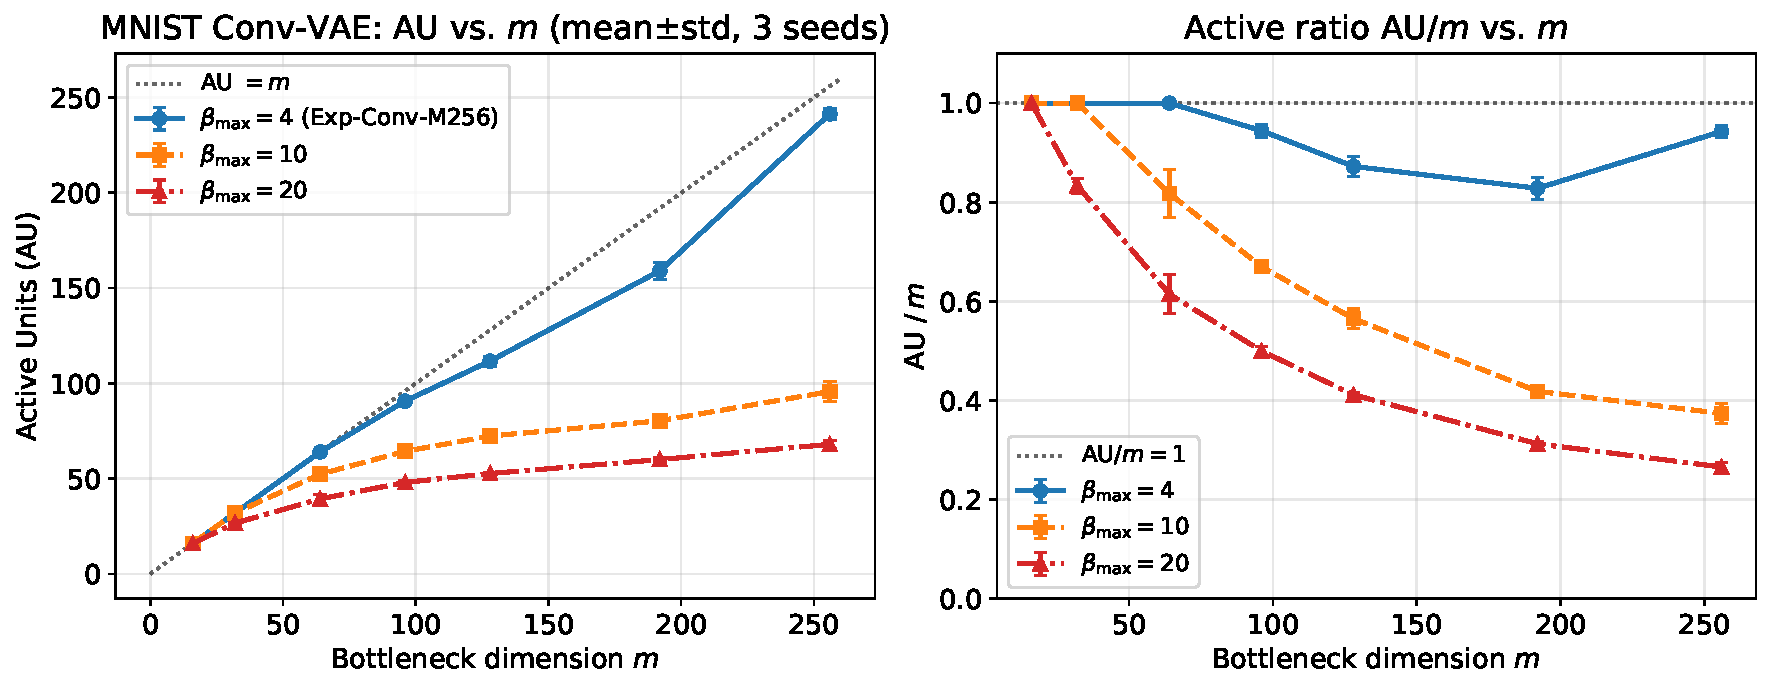
\includegraphics[width=0.9\linewidth]{results/figures/Exp_ConvV_HiBeta.pdf}
\caption{Exp-ConvV-HiBeta (mean$\pm$std, 3 seeds): increasing
$\beta_{\max}$ shifts the AU truncation to lower dimensions, consistent with
the surrogate activation condition.}
\label{fig:hibeta}
\end{figure}}{}

\subsection[\appendixname~\thesubsection]{Search for AU Plateaus on Natural Images (Exp-NatImg-Sweep)}

In a sweep of the CIFAR-10 Conv-VAE combining $m \in [32, 1024]$,
$\beta_{\max} \in \{10, 20, 40, 80\}$, and decoder capacities
(Standard/Deep/Thin), plateau-like behavior of AU around $\approx 24$ was
observed over $m \in [512, 1024]$ under the condition
$\beta_{\max} = 80$ with a thin decoder (preliminary evidence).
Across all conditions the latent TwoNN remained stable at $24.7$--$25.4$,
consistent with Pope et al.~\cite{pope2021intrinsic}.
Stable identification including seed and grid stability is unmet and remains
future work.

\subsection[\appendixname~\thesubsection]{Preliminary VAE Observation on Fashion-MNIST (Exp-Fashion)}

This is the preliminary observation that preceded the 3-seed verification
(Exp-Fashion-MS) of Section~\ref{sec:exp_fashion}.
For the Fashion-MNIST VAE ($\beta = 4$, 100 epochs, single seed), the AE
side TwoNN converges to $\approx 9.4$ for $m_{\mathrm{ref}} \geq 32$ (the
grid-design value $d = 9$ of Exp-Real-Geom is based on this preliminary
estimate), and an AU slowdown region of the same order as
$\hatdID \approx 9$--10 was observed (same tendency as MNIST).
This preliminary observation has been superseded by Exp-Fashion-MS
(3 seeds, 300 epochs; Section~\ref{sec:exp_fashion}), where a V1 pass with
a violation of the lower V2 bound was confirmed consistently across the 3
seeds.

\subsection[\appendixname~\thesubsection]{$\AUsat$ on Topological Manifolds (Exp-Syn-Top)}

On the Torus and the M\"obius band (both $\dID = 2$, $\demb = 3$) we
observed $\AUsat = 3 = \demb$, and on the circle $S^1$ ($\demb = 2$)
$\AUsat = 2$ (for $m \geq 6$, conditional).
The $\AUsat$ of the Swiss Roll depends on preprocessing (2 with
standardization, 3 otherwise), so the main evidence for the
$\AUsat = \demb$ correspondence is limited to the Torus and M\"obius band.
This is a conditional incidental observation with no claim of theoretical
necessity.

\section[\appendixname~\thesection]{Sensitivity Analyses and Experiment Overview}\label{app:sens}

\textbf{AU threshold $\delta$}: AU values are essentially unchanged for
$\delta \in [10^{-3}, 10^{-1}]$ (MNIST FC-VAE, 300 epochs).

\textbf{$\beta$ sensitivity}: in preliminary experiments (50 epochs,
$\beta \in \{1, 2, 4, 8\}$), $\beta = 1$ gives AU $\approx m$
(under-regularization) and $\beta = 8$ shows signs of over-regularization;
AU patterns are stable for $\beta \in [2, 8]$.
The default $\beta = 4$ of this paper is the center of this stable range.

\textbf{$k$ sensitivity of MLE}: MLE $= 11.5$--12.4 (MNIST) for
$k \in \{5, 10, 20\}$, stable.

\begin{table}[H]
\caption{Experiment overview. Main-text VAE verification results used for
the principal verdicts use 3 seeds (42, 123, 777); single-seed sweeps are
marked in the Seeds column; appendix experiments marked ``single'' use
seed 42 only.}
\label{tab:exp_list}
\small
\begin{tabular}{p{3.2cm}p{3.4cm}p{1.4cm}p{1.2cm}p{2.4cm}}
\toprule
\textbf{Experiment} & \textbf{Data / model} & \textbf{Epochs} & \textbf{Seeds} & \textbf{Section} \\
\midrule
Exp-Syn-1 / Exp-Syn-AU & Swiss Roll, Torus / AE, VAE & 200--300 & 3 & Section~\ref{sec:exp_syn} \\
Exp-Syn-Verify & Torus, Swiss Roll / VAE ($m = 3$--$8$) & 200 & 5 & Section~\ref{sec:exp_syn} \\
Exp-Mnist-Base & MNIST / AE ($m_{\mathrm{ref}}$ sweep) & 300 & 1 (sweep) & Section~\ref{sec:exp_mnist} \\
Exp-Mnist-Multi-300 & MNIST / FC-VAE & 300 & 3 & Section~\ref{sec:exp_mnist} \\
Exp-Mnist-Dense-300 & MNIST / FC-VAE (dense grid) & 300 & 3 & Section~\ref{sec:exp_mnist_dense} \\
Exp-Boot-CI & MNIST / ref.-AE latents (re-analysis) & --- & subsamp. & Section~\ref{sec:exp_mnist_ci} \\
Exp-Downstream & MNIST / AE probe, FC-VAE probe & 300 & 1 (AE), 3 (VAE) & Section~\ref{sec:exp_downstream} \\
Exp-Real-Geom & MNIST, F-MNIST / AE, IsoAE, CAE, DAE & 300 & 3 & Section~\ref{sec:exp_real_geom} \\
Exp-Conv-M256 / M512 & MNIST / Conv-VAE & 150 & 3 & Section~\ref{sec:exp_boundary} \\
Exp-Nat-Cifar / Exp-Nat-SVHN & CIFAR-10, SVHN / Conv-VAE & 150 & 3 & Section~\ref{sec:exp_boundary} \\
Exp-Fashion-MS & F-MNIST / FC-VAE & 300 & 3 & Section~\ref{sec:exp_fashion} \\
Exp-ConvV-HiBeta & MNIST / Conv-VAE ($\beta_{\max}$ up) & 150 & 3 & App.~\ref{app:exploratory} \\
Exp-NatImg-Sweep & CIFAR-10 / Conv-VAE & 300 & partial & App.~\ref{app:exploratory} \\
Exp-Fashion & F-MNIST / AE, VAE (preliminary) & 100 & single & App.~\ref{app:exploratory} \\
Exp-Syn-Top & Torus, M\"obius, $S^1$ / VAE & 300 & single & App.~\ref{app:exploratory} \\
\bottomrule
\end{tabular}
\end{table}

%%%%%%%%%%%%%%%%%%%%%%%%%%%%%%%%%%%%%%%%%%
\begin{thebibliography}{999}

\bibitem{kingma2014vae}
Kingma, D.P.; Welling, M.
Auto-encoding variational Bayes.
In \textit{International Conference on Learning Representations (ICLR)},
2014.

\bibitem{bengio2013representation}
Bengio, Y.; Courville, A.; Vincent, P.
Representation learning: A review and new perspectives.
\textit{IEEE Trans.\ Pattern Anal.\ Mach.\ Intell.} \textbf{2013},
\textit{35}, 1798--1828.

\bibitem{lucas2019elbo}
Lucas, J.; Tucker, G.; Grosse, R.B.; Norouzi, M.
Don't blame the ELBO! A linear VAE perspective on posterior collapse.
In \textit{NeurIPS 2019}, Vol.~32, 2019.

\bibitem{fefferman2016manifold}
Fefferman, C.; Mitter, S.; Narayanan, H.
Testing the manifold hypothesis.
\textit{J.\ Am.\ Math.\ Soc.} \textbf{2016}, \textit{29}, 983--1049.

\bibitem{facco2017twonn}
Facco, E.; d'Errico, M.; Rodriguez, A.; Laio, A.
Estimating the intrinsic dimension of datasets by a minimal neighborhood
information.
\textit{Sci.\ Rep.} \textbf{2017}, \textit{7}, 12140.

\bibitem{pope2021intrinsic}
Pope, P.; Zhu, C.; Abdelkader, A.; Goldblum, M.; Goldstein, T.
The intrinsic dimension of images and its impact on learning.
In \textit{ICLR 2021}, 2021.

\bibitem{ansuini2019intrinsic}
Ansuini, A.; Laio, A.; Macke, J.H.; Zoccolan, D.
Intrinsic dimension of data representations in deep neural networks.
In \textit{NeurIPS 2019}, Vol.~32, 2019.

\bibitem{valeriani2023geometry}
Valeriani, L.; Wood, D.; Catania, G.; Gherardini, S.; Laio, A.; Ansuini, A.
The geometry of hidden representations of large transformer models.
In \textit{NeurIPS 2023}, Vol.~36, 2023.

\bibitem{higgins2017betavae}
Higgins, I.; Matthey, L.; Pal, A.; Burgess, C.; Glorot, X.; Botvinick, M.;
Mohamed, S.; Lerchner, A.
$\beta$-VAE: Learning basic visual concepts with a constrained variational
framework.
In \textit{ICLR 2017}, 2017.

\bibitem{alain2014dae}
Alain, G.; Bengio, Y.
What regularized auto-encoders learn from the data-generating distribution.
\textit{J.\ Mach.\ Learn.\ Res.} \textbf{2014}, \textit{15}, 3743--3773.

\bibitem{rifai2011cae}
Rifai, S.; Vincent, P.; Muller, X.; Glorot, X.; Bengio, Y.
Contractive auto-encoders: Explicit invariance during feature extraction.
In \textit{ICML 2011}, Vol.~28, 2011.

\bibitem{birdal2021intrinsic}
Birdal, T.; Lou, A.; Guibas, L.J.; Simsekli, U.
Intrinsic dimension, persistent homology and generalization in neural
networks.
In \textit{NeurIPS 2021}, Vol.~34, 2021.

\bibitem{levina2005mle}
Levina, E.; Bickel, P.J.
Maximum likelihood estimation of intrinsic dimension.
In \textit{Advances in Neural Information Processing Systems (NeurIPS)},
Vol.~17, 2005.

\bibitem{ceruti2014danco}
Ceruti, C.; Bassis, S.; Rozza, A.; Lombardi, G.; Casiraghi, E.;
Campadelli, P.
DANCo: An intrinsic dimensionality estimator exploiting angle and norm
concentration.
\textit{Pattern Recognit.} \textbf{2014}, \textit{47}, 2569--2581.

\bibitem{camastra2016intrinsic}
Camastra, F.; Staiano, A.
Intrinsic dimension estimation: Advances and open problems.
\textit{Inf.\ Sci.} \textbf{2016}, \textit{328}, 26--41.

\bibitem{allegra2020data}
Allegra, M.; Facco, E.; Denti, F.; Laio, A.; Mira, A.
Data segmentation based on the local intrinsic dimension.
\textit{Sci.\ Rep.} \textbf{2020}, \textit{10}, 16449.

\bibitem{tippingbishop1999ppca}
Tipping, M.E.; Bishop, C.M.
Probabilistic principal component analysis.
\textit{J.\ R.\ Stat.\ Soc.\ Ser.\ B} \textbf{1999}, \textit{61}, 611--622.

\bibitem{bishop1999bayesian}
Bishop, C.M.
Bayesian PCA.
In \textit{Advances in Neural Information Processing Systems}, Vol.~11,
1999; pp.~382--388.

\bibitem{ghahramani2005infinite}
Ghahramani, Z.; Griffiths, T.L.
Infinite latent feature models and the Indian buffet process.
In \textit{Advances in Neural Information Processing Systems}, Vol.~18,
2005.

\bibitem{nazari2023geometric}
Nazari, P.; Damrich, S.; Hamprecht, F.A.
Geometric autoencoders---what you see is what you decode.
In \textit{ICML 2023}, \textit{PMLR} Vol.~202.

\bibitem{kato2020rdae}
Kato, K.; Zhou, J.; Sasaki, T.; Nakagawa, A.
Rate-distortion optimization guided autoencoder for isometric embedding in
Euclidean latent space.
In \textit{ICML 2020}, \textit{PMLR} Vol.~119.

\bibitem{hatcher2002algebraic}
Hatcher, A.
\textit{Algebraic Topology};
Cambridge University Press: Cambridge, UK, 2002.

\bibitem{lecun1998}
LeCun, Y.; Bottou, L.; Bengio, Y.; Haffner, P.
Gradient-based learning applied to document recognition.
\textit{Proc.\ IEEE} \textbf{1998}, \textit{86}, 2278--2324.

\bibitem{xiao2017fashion}
Xiao, H.; Rasul, K.; Vollgraf, R.
Fashion-{MNIST}: A Novel Image Dataset for Benchmarking Machine Learning
Algorithms.
\textit{arXiv} \textbf{2017}, 1708.07747.

\bibitem{kornblith2019cka}
Kornblith, S.; Norouzi, M.; Lee, H.; Hinton, G.
Similarity of neural network representations revisited.
In \textit{ICML 2019}, Vol.~97, pp.~3519--3529, 2019.

\bibitem{johnsson2015ess}
Johnsson, K.; Soneson, C.; Fontes, M.
Low bias local intrinsic dimension estimation from expected simplex
skewness.
\textit{IEEE Trans.\ Pattern Anal.\ Mach.\ Intell.} \textbf{2015},
\textit{37}, 196--202.

\bibitem{fu2019cyclical}
Fu, H.; Tan, C.; Peng, B.; Zhao, Z.; Yan, T.; Chang, C.; Zhao, L.
Cyclical annealing schedule: A simple approach to mitigating {KL} vanishing.
In \textit{Proceedings of NAACL-HLT 2019}, Minneapolis, MN, USA, 2019;
pp.~240--250.

\bibitem{krizhevsky2009learning}
Krizhevsky, A.
Learning multiple layers of features from tiny images.
\textit{Technical Report}, University of Toronto, 2009.

\bibitem{netzer2011reading}
Netzer, Y.; Wang, T.; Coates, A.; Bissacco, A.; Wu, B.; Ng, A.Y.
Reading digits in natural images with unsupervised feature learning.
In \textit{NIPS Workshop on Deep Learning and Unsupervised Feature Learning},
2011.

\bibitem{sonderby2016ladder}
S{\o}nderby, C.K.; Raiko, T.; Maal{\o}e, L.; S{\o}nderby, S.K.; Winther, O.
Ladder variational autoencoders.
In \textit{Advances in Neural Information Processing Systems (NeurIPS)},
Vol.~29, 2016.

\bibitem{cover2006elements}
Cover, T.M.; Thomas, J.A.
\textit{Elements of Information Theory}, 2nd ed.;
Wiley-Interscience: Hoboken, NJ, USA, 2006.

\bibitem{hoffman2016elbo}
Hoffman, M.D.; Johnson, M.J.
{ELBO} surgery: Yet another way to carve up the variational evidence lower
bound.
In \textit{NIPS Workshop on Advances in Approximate Bayesian Inference},
2016.

\end{thebibliography}

\end{document}
